\chapter{From surface phonological tone to phonetic realization}
\label{chap:fromsurfacephonologicalformstophoneticrealizationintonationandtonalimplementation}

\epigraph{{\dots}~a~theory of tone must provide some means for describing intonational processes independently of tonal patterns, as well as a~procedure for integrating the two structures.}{\citep[547]{clements1979}}

\epigraph{If, as seems to be the case, the complexity of \isi{intonation} is typical of human complexity, then there is still a~long way to go before ({\dots}) \isi{intonation} yields all of its secrets.}{\citep[256]{vaissiere2004}}

\is{phonetic realization of tones|(}

\section{Introduction}
\label{sec:introductionsurfacetoreal}

The established order of business when describing a~language is to elucidate the phonological and morphophonological facts first, and to address issues of phonetic implementation later. In practice, tones and \isi{intonation} are necessarily studied together, since they share an~all"=important phonetic
correlate: voice fundamental frequency (F\textsubscript{0}). This is especially clear in
languages such as Na, where tones are specified only in terms of pitch: in Na, unlike in
many other East/Southeast Asian languages, tones do not
have length or phonation"=type characteristics as part of their phonological definition. (This topic is taken up in the typological discussion, \sectref{sec:typologicalbackgroundtotheclassificationofyongningnatonesasleveltones}.)

This chapter contains observations about the phonetic implementation of tone, and \isi{intonation} in general: everything that happens when surface phonological\is{form!surface} tone translates into a~concrete phonetic realization. 

As an~introduction to this domain, \figref{fig:spectrogramandf0tracingoftwonaphrases} shows spectrograms of /\ipa{bo˩-ɬv̩˧˥}/ ‘pig’s brains’ and /\ipa{bo˩-ɬv̩˧} \ipa{ɲi˥}/
‘is \mbox{(a/the)} pig’s brains’. 

\begin{figure}
\includegraphics[width=.70\textwidth]{figures/PigBrains/PigBrains.eps}
\caption{\label{fig:spectrogramandf0tracingoftwonaphrases}Spectrogram and F\textsubscript{0} tracing of  ‘pig’s brains’ and ‘is \mbox{(a/the)} pig’s brains’.}
\end{figure}


The clear rise in F\textsubscript{0} on the rhyme /\ipa{v̩}/ in the top part of the figure is consistent with
phonological description as a~MH tone; and the flatter shape on the same rhyme in the bottom part
of the figure, followed by higher F\textsubscript{0} on the \isi{copula}, is consistent with phonological description as
a~sequence of M on one syllable and H on the next. But there is no way to read phonological tones off F\textsubscript{0}
tracings (as emphasized e.g.~by \citealt{cruzetal2014} and \citealt{morey2014}). \figref{fig:spectrogramandf0tracingoftwonaphrases} illustrates a~phenomenon that is immediately apparent when examining any
piece of \is{experimental phonetics|textbf}experimental evidence: variability in the realization of tone. For instance,
glottalization, which is common in Yongning Na in utterance"=final position, is found at the end of both tokens, exerting a~lowering influence on F\textsubscript{0}
towards the offset of voicing. (In these materials, the phrases /\ipa{bo˩-ɬv̩˧˥}/ ‘pig’s brains’ and /\ipa{bo˩-ɬv̩˧ ɲi˥}/ ‘is
(a/the) pig’s brains’ are both found in absolute final position, and therefore constitute entire sentences on
their own.) Also, /\ipa{bo˩}/
‘pig’ is realized with noticeably different F\textsubscript{0} in the top part of the figure and in the bottom
part. Tone levels have some range of \isi{variation} within tonal space (F\textsubscript{0}), in the same way as vowels have some
range of \isi{variation} within the acoustic space (as characterized essentially by the first three
formants, F1-F2-F3). In Yongning Na, rising tones are never found in initial position within a~tone
group, and hence the identification of an~initial L tone (as on the syllable /\ipa{bo˩}/ ‘pig’) is not jeopardized
by its realization with a~slight rise, as in the top part of \figref{fig:spectrogramandf0tracingoftwonaphrases}. Seen in this light, the
existence of slightly rising allotones (allophones of the tones) does not come as a~surprise: it makes sense in view of the
state of the phonological system, in the same way as, in a~language that does not have contrastive aspirated
consonants, plain (unaspirated) unvoiced consonants may sometimes be realized phonetically with some
aspiration.

Back in the 1970s, at a~time when F\textsubscript{0} tracings were difficult to do, necessitating expert technical skill, a~specialist in Bantu tone asked a~phonetician to create an~F\textsubscript{0}
tracing from a~recording illustrating a~specific phonological phenomenon. After receiving the
desired tracing, this famous specialist of tonology said that there must be a~mistake, as the F\textsubscript{0}
tracing did not correspond to the tone pattern that his trained ear discerned clearly in the
recording. In fact, there was no error in F\textsubscript{0} detection: the issue lay in this colleague’s
expectation of a~neatly binary F\textsubscript{0} tracing, straightforwardly reflecting the phonological tone
sequence (J. Vaissière, p.c.\ 2001). Experimental examination of spoken language reveals that, even in languages with
relatively straightforward prosodic systems, such as Standard \ili{Japanese}, F\textsubscript{0} curves are shaped by
a~number of factors, and do not reflect phonological tone in a~crystal"=clear, transparent
way. Without the help of a~language consultant, it is simply impossible to know for sure for a~given
utterance that has, for instance, a~lowering of F\textsubscript{0} on its last
syllable, whether this is due to a~L tone on that syllable or to intonational final lowering of
a~M-tone syllable. Arriving at tonal contrasts requires factoring out \isi{intonation}, and vice versa.


The following sections present salient characteristics of Na \isi{intonation}. But first some concepts need
to be discussed.




\subsection{Definition of terms}
\label{sec:definitionofterms}

\is{prosody|textbf}Prosody as defined here consists of (i)~lexically distinctive properties: stress, as in
\ili{English}; tone, as in \ili{Mandarin}, Yorùbá or Na; tonal accent, as in \il{Japanese|textbf}Japanese\footnote{As mentioned in \sectref{sec:adiscussionofalternativeformulations}, several competing analyses of the prosodic systems of {Japanese} dialects have been proposed (for a~review, see \citealt{kawahara2015}). The concept of tonal accent, also called pitch accent, has been presented by \citet{hymanhownot2009} as a~typical example of how \textit{not} to do prosodic typology: the argument is that “alleged pitch"=accent systems freely pick"=and"=choose properties from the tone and stress prototypes, producing mixed, ambiguous, and sometimes analytically indeterminate systems which appear to be intermediate”. However, the description of pitch"=accent systems as “intermediate” between stress and tone does not greatly clarify the issue. Hyman's questioning of pitch accent as a~typological category could be extended to tone, in view of the considerable heterogeneity of prosodic systems that have been described as “tone systems” (see \citealt{brunelleetal2016} and the discussion
	 in \sectref{sec:typologicalbackgroundtotheclassificationofyongningnatonesasleveltones}). As Hyman underlines, the goal of prosodic typology should be to classify not languages but rather the properties of their subsystems. In the present state of prosodic typology, it is not obvious to me that there is much to gain from prohibiting tonal accent as a~descriptive label.} and Swedish;
phonation"=type register, as in Mon (\il{Mon-Khmer}Mon"=Khmer family); (ii)~\isi{intonation}; and (iii)~performance
factors, including rhythm.

\is{intonation|textbf}Intonation is often identified with the parameters in which
it is manifested~-- and especially with fundamental frequency. But this identification is inappropriate, because intonation is a~complex, abstract
structure. It can usefully be divided into (i)~two sub"=systems of linguistic structure: syntactic
\isi{intonation} \textit{(\isi{phrasing})}, which essentially reflects syntax in the broader sense, and pragmatic
\isi{intonation} \textit{(prominence)}, which reflects \isi{information structure}, and (ii)~attitudinal and emotional
dimensions, which convey speaker attitudes and emotions. This view of \isi{intonation} is shown in \figref{fig:intonation}. It needs to be emphasized that this embedded (tree"=like) graph is a~highly simplified representation: its aim is to provide a~visual recapitulation of the basic distinctions made here. It does not aim to reflect the delicate links among the various components of \isi{prosody}, e.g.~between rhythm and lexically distinctive suprasegmentals.

\begin{figure}[ht]
	\centering
	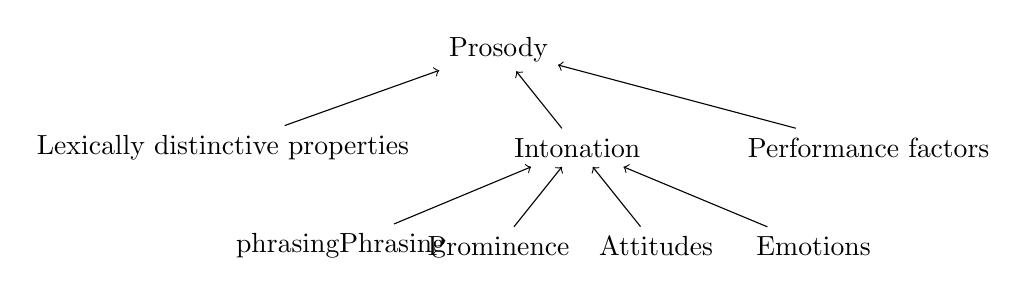
\begin{tikzpicture}
%	\node (a) at (0, 1) {\textsc{gen/num (erg)}};
	\node (b) at (1.5, 1.5) {\is{phrasing}Phrasing};
%	\node (c) at (1.5, 2.5) {\textsc{gen/num (erg)}};
	\node (d) at (0, 2.75) {Lexically distinctive properties};
	\node (e) at (3.5, 1.5) {Prominence};
%	\node (f) at (3, 1) {\textsc{gen/num (erg)}};
	\node (g) at (4.5, 2.75) {Intonation};
	\node (g2) at (8.2, 2.75) {Performance factors};
	\node (h) at (5.5, 1.5) {Attitudes};
	\node (i) at (7.5, 1.5) {Emotions};
%	\node (j) at (6, 1) {\textsc{gen/num (acc)}};
%	\node (k) at (9, 1) {\textsc{person (acc)}};
%	\node (l) at (9, -0.5) {Past \textit{\textbf{(Past Imperfect)}}};
%	\node (m) at (9, -1) {\textsc{person (acc)}};
	\node (n) at (3.5, 4) {Prosody};
	\foreach \from/\to in {g/h, g/i, n/d, n/g, g/b, g/e, n/g2}
	\draw [<-] (\from) -- (\to);
	\end{tikzpicture}
	\caption{A highly schematic representation of the components of {prosody}.}
		\label{fig:intonation}
\end{figure}

%\begin{figure}[h!]
%	\caption[{A highly schematic representation of the components of \isi{prosody}.}]{A highly schematic representation of the components of \isi{prosody}.}
%
%\begin{tikzpicture}
%
%[sibling distance=10em,
%every node/.style = {shape=rectangle, rounded corners,
%	draw, align=center,
%	top color=white, bottom color=blue!20}]
%
%\node {prosody} % 1st level. No need for closing.
%		child { node {lexically distinctive properties} %2nd level, 1st branch OPENED
%%					child { node {tone (as in Na)} }
%%					child { node {stress (as in \ili{English})} }
%%					child { node {tonal accent (as in \ili{Japanese})} }
%%					child { node {phonation"=type registers (as in Mon)} }
%			} % 2nd level, 1st branch CLOSED
%		child { node {intonation} %2nd level, 2nd branch OPENED
%%					child { node {linguistic\\ structuration\\ systems} %3rd level, 1st branch
%						child { node {phrasing} }
%						child { node {prominence} }
%					%		child { node {center} } }
%%					 } % %3rd level, 1st branch CLOSED
%%				 	child { node {attitudinal\\ and\\ emotional\\ dimensions}  %3rd level, 2nd branch OPENED
%				 		child { node {attitudes} }
%				 		child { node {emotions} }
%				 		%		child { node {center} } }
%%				 	} %3rd level, 2nd branch CLOSED
%				child { node {performance\\ factors} }
%		; % semicolon to close the list of nodes
%
%\end{tikzpicture}
%\end{figure}

These definitions, taken from a~publication about prosodic constituents in \ili{French}
\citep{vaissiereetal2006}, elaborate on proposals which (in my view) are similar in their essentials
\citep{coustenobleetal1937,delattre1965,martin1977b,rossi1999}. Usage
still varies considerably among authors (a detailed discussion of various frameworks is proposed
by \citealt{dicristo1998}).

As defined here, tone has the function of lexical and morphological differentiation, and
\isi{intonation} has the functions of (i)~speech \isi{phrasing}, (ii)~coding prominence, and (iii)~expressing emotions and attitudes towards the listener. Intonation is, in Bolinger’s phrase, a~“half"=tamed savage”
\citep[475]{bolinger1978}. \textit{Phrasing} is on the tamer, more intellectual side; it surfaces at
its clearest in deliberate oral renderings of elaborately composed texts. \textit{Prominence} is
a~less tame dimension of \isi{intonation}: it can still be described in terms of a~linguistic system, with
clear cross"=linguistic differences, but the intrusion of the stronger manifestations of prominence
can interfere with \isi{phrasing} as determined by syntactic structure. The expression of attitudes
and emotions can partly be described in terms of ethological principles, such as the Frequency Code:
 
\begin{quotation}
{\dots}~an innately specified ‘Frequency
Code’ ({\dots}) associates high acoustic frequency with the primary meaning of ‘small vocalizer’ and thus secondary meanings as ‘subordinate, submissive, non threatening, desirous of the receiver's goodwill, etc.’ and associates with low acoustic frequency the primary meaning of ‘large vocalizer’ and such secondary meanings as ‘dominant, aggressive, threatening’, etc.~ \citep[1]{ohala1984}.
\end{quotation}
	
The phrase “syntactic \isi{intonation}” may appear to be somewhat of a~misnomer, insofar as intonational \isi{phrasing} does not stand in a~strict, one"=to"=one relationship with syntactic units, as was
already noted in the early classics of phonetics \citep{grammont1933} and confirmed by later work
(\citealt{selkirk1972}; \citeyear[231]{selkirk2000}; \citealt{martin1981}). The phrase “syntactic
\isi{intonation}” is nonetheless retained in view of the fact that knowledge of a~sentence’s syntax offers
a~sufficient basis for the synthesis of an~acceptable fundamental frequency {contour}
\citep{vaissiere1971}.

The acoustic correlates of \isi{prosody} are many. They include the variations in fundamental frequency,
\isi{duration} and intensity and \is{phonation types}phonation type, but also the allophonic variations in the realization of
the phonemes. Thus, \isi{prosody} has correlates at the respiratory level (i.e.\ the subglottal level), at the glottis,
and at the supra"=glottal level (see \citealt{erickson1998}). All parameters take part in \isi{prosody} simultaneously, to a~greater or
lesser extent.

Lastly, here are some clarifications about the concepts of ‘\isi{tone sandhi}’, ‘morphotonology’ and ‘tonal morphology’. \is{tone sandhi|textbf}\textit{Tone sandhi} refers to phonologically specified tone change, applying automatically inside a~given phonological domain. To put it differently, \textit{tone sandhi} refers to categorical phenomena of tone change conditioned by the phonological context. The seven tonal rules of Yongning Na presented in \sectref{sec:alistoftonerules} (repeated below) are \isi{tone sandhi} rules, in the sense that they govern adjustments among neighbouring tones within a~given phonological domain (the \isi{tone group}).

	\begin{enumerate}[leftmargin=2cm, itemsep=0pt, labelwidth=\widthof{Rule~1:}]%[topsep=12pt, partopsep=0pt]
		\item[Rule~1:] L tone spreads progressively (“left"=to"=right”) onto syllables that are unspecified for tone.
		\item[Rule~2:] Syllables that remain unspecified for tone after the application of Rule 1 receive M tone.
		\item[Rule~3:] In tone"=group"=initial position, H and M are neutralized to M.
		\item[Rule~4:] The syllable following a~H-tone syllable receives L tone.
		\item[Rule~5:] All syllables following a~H.L or M.L sequence receive L tone.
		\item[Rule~6:] In tone"=group"=final position, H and M are neutralized to H if they follow a~L tone.
		\item[Rule~7:] If a~\isi{tone group} only contains L tones, a~post"=lexical H tone is added to its last syllable.
	\end{enumerate}

\textit{Morphotonology} refers to categorical change in tone governed by rules that are confined to specific syntactic phrase types, e.g.~the different rules that apply to object plus verb, subject plus verb, numeral plus classifier, and so on. 

Finally, \textit{tonal morphology} refers to grammatically specified tone change marking certain morphosyntactic categories. The phrase “tone cases” is used in the description of some \ili{Bantu} languages, such as UMbundu \citep{schadeberg1986tone}, where a~noun's tone changes according to its case. 
%No less than twenty"=five African languages that have tone cases are listed (and plotted on a~map) by \citet[225]{konig2008case}. 
The addition of a~certain tone to verbs can express a~given tense/aspect/modality category. 
%Tonal morphology can further be divided into \textit{concatenative} and \textit{derivational} types. Concatenative tonal morphology consists in the addition of “tonal morphemes” (on the case of Saramaccan: \citealt{good2002, good2004}). 

In Yongning Na, there is no tonal morphology, in the sense that there are no tonal morphemes. The \is{floating tone}floating High tone in Yongning Na is not a~morpheme (the combination of a~form and a~meaning): it is one of the lexical categories of nouns. As a~consequence, only the first two of the three concepts characterized above~-- \is{tone sandhi}sandhi, morphotonology, and tonal morphology~-- are relevant to the present study. 

Some authors prefer “a broad and loose usage of the term” \textit{sandhi} covering both \is{tone sandhi}sandhi and morphotonology as defined here \citep[x]{chen2000}. But while it is advisable to cast the net wide in language surveys \citep[such as the survey of Chinese dialects by][]{chen2000}, the distinction between sandhi and morphotonology is crucial to the present study. The reason for writing a~book"=length description is that tonal changes in Yongning Na are not simply a~matter of phonology: in addition to sandhi (as defined here: a~phonological phenomenon), Yongning Na has a~host of syntactically restricted \is{tone rules}tone rules, i.e.\ morphotonology. 


\subsection[About tools for intonational transcription]{About tools for intonational transcription}
\label{sec:theabsenceoffullysatisfactorytoolsforintonationaltranscription}

There does not yet exist a~standardized system for transcribing \isi{intonation}. This is easy to
understand in view of the intricacy of this linguistic domain, described above. 

\begin{quotation}
	Since Bolinger first raised the {question} explicitly in \citeyear{bolinger1951}, there has been considerable argument over whether \isi{intonation} is better described as pitch contours, like the kinetic tones of the British tradition, or as a~sequence of pitch phonemes or significant levels (the American approach exemplified by \citealt{pike1945}, \citealt{wells1945}, \citealt{trageretal1951}, \citealt{hockett1955}, and now \citealt{liberman1975} and the autosegmental school originated by \citealt{goldsmith1976}). \citep[531]{ladd1978}
\end{quotation}

%Command \noindent added to avoid having an indent. Proofreader suggestion: since this sentence continues the argument, it is better not to indent. 
{\noindent}Under the second of these approaches, \isi{intonation} is modelled by means of discrete levels, as if it were tonal. This approach is known as “autosegmental"=metrical”, and has dominated
discussions of \isi{intonation} since the 1980s. A~reason for its popularity is that it seemed to hold promise for implementation in speech synthesis \citep{pierrehumbert1981} and prosodic annotation \citep{silvermanetal1992}. The basic tenets of “autosegmental"=metrical” models are concepts borrowed from autosegmental tonology, such as level
tones, \isi{downstep} and tone \is{tone spreading}spreading. Pitch accents, organized in a~linear sequence, are considered the building blocks of an \isi{intonation} {contour} (see the textbooks by \citealt{ladd1996} and \citealt{gussenhoven2004}, for instance).

If one stands back to take a~global view of tonal models of \isi{intonation}, however, they appear as hybrid and
somewhat perplexing systems (as pointed out by \citealt{martin2001} and \citealt{wightman2002}). The posited ‘intonational tones' are abstract
entities, but the labels are also used as a~system for phonetic transcription of linguistically
significant aspects of F\textsubscript{0} curves as they are observed. Tonal labels tend to be assigned by eye (on the basis of F\textsubscript{0} curves superimposed on spectrographic displays) more than by ear,
whereas ‘\isi{boundary tone}s' are meant to reflect the perceived cohesion between successive words, and
are thus grounded in aural impressions as well as on the observation of F\textsubscript{0} curves. “To be fair to the original spirit of Janet Pierrehumbert, who intended to describe
American \ili{English} and carefully avoided generalization in her thesis, applying ToBI symbols to a~new
language requires prior re"=evaluation of the underlying principles” \citep{vaissiere2002}.

Interestingly, before he became one of the proponents of “autosegmental"=metrical” models, Bob Ladd expressed the conviction that he had “clearly demonstrate[d] the inadequacy of any approach to \ili{English} \isi{intonation} which treats contours as sequences of significant pitch levels” \citep[517]{ladd1978}.

\begin{quotation}
	In short, linguistic systems force users to identify certain signals as discretely different from one another; and linguists' analyses should reflect these discrete differences. But an analysis of \isi{intonation} in terms of pitch levels forces us to distinguish points along a~gradient as also being discretely different~-- even though they are not~-- because the theory provides no principled way of knowing when changing a~certain feature in a~sequence is going to produce a~‘modulation’, and when it is going to produce a~‘very different tune’. No amount of tinkering with theoretical mechanisms can remedy this defect; the best that any pitch-level theory can do is ignore it. To continue to ignore the difference between the gradient and the all"=or"=none by forcing it into a~pre"=ordained system of distinctions is only to put off reaching an understanding of how \isi{intonation} really functions in language. \citep[539]{ladd1978}
\end{quotation}

%Command \noindent added to avoid having an indent. Proofreader suggestion: since this sentence continues the argument, it is better not to indent. 
{\noindent}This strand of thought (which makes excellent sense to me) continued to be pursued by some scholars even during the heyday of “autosegmental"=metrical” models. Alternatives to tonal models of \isi{intonation} include the Kiel Intonation Model and its developments
\citep{niebuhretal2004,kohler2005,niebuhr2007,Niebuhr2010}, superpositional approaches
\citep{vaissiere2002,vaissiere2004,gronnum1991,gronnum1998a,gronnum1998b,lindau1986}, and various others \citep{delattre1966a,fonagy1989,rossi1999,martin1977b,martin2015,hirstetal1998b}. These approaches are currently
outside the mainstream of \isi{intonation} studies, in the same way as non"=autosegmental analyses of tone
systems fall outside mainstream (generative) phonology (some reflections on this situation are set
out in \citealt{zerbian2010,michaudetal2015f}). My evaluation of the available evidence is
that tonal accounts of \isi{intonation} in tone languages run into considerable difficulties, and that it
is better to adopt a~vocabulary which suits the data, even if it is not mainstream at present,
rather than force the data into inadequate models. As a~consequence, the
present description adopts a~functional
perspective that clearly distinguishes tone and \isi{intonation}.

Another distinction which is essential to \isi{prosody} studies is that between an~abstract level of description, on the one hand, and the level of phonetic realizations, on the other. This distinction is threatened in frameworks where ‘tone’
  is considered synonymous with F\textsubscript{0}. For instance, \citet{hymanetal2008b} define the term ‘tonal’ in a~phonetic sense, to mean
  ‘realized by F\textsubscript{0}’, and ‘non"=tonal’ to mean ‘realized by parameters other than F\textsubscript{0}’ (such as
  phonation types). The equation between ‘tone’ and ‘F\textsubscript{0}’ appears so self"=evident that it could seem unnatural to try to define tone in any different
  way. But from a~classical linguistic perspective, it is crucial to make a~distinction between
  F\textsubscript{0}, which is an~acoustic parameter, and linguistic tone, which is a~functional concept.


\subsection{Intonation in level"=tone languages: A~review}
\label{sec:literaturereviewintonationintonallanguages}

In addition to the above remarks about the definition of terms and the frameworks for studying \isi{intonation}, it may be useful, before beginning to describe \isi{intonation} in Yongning Na, to review studies of \isi{intonation} in other level"=tone languages. This review also paves the way for the typological analyses set out in a later chapter (\sectref{sec:typologicalperspectives}).

Auditory observations on phonetic realizations of tone in a~two"=tone language (Lingala) are proposed by \citet{guthrie1940}:

\begin{quotation}
	{\dots}~the only possible variations in the \isi{intonation} of a~word or sentence are these: 
	\begin{enumerate}[itemsep=0pt, topsep=0pt, partopsep=0pt, parsep=0pt]
	\item[(a)] A~widening or narrowing of the interval between the high and the normal tones.
	\item[(b)] A~raising or lowering of the pitch of voice, i.e.\ a~change of key.
	\item[(c)] A~gradual rise or fall of the pitch of voice, i.e.\ a~continuous change of key.
	\end{enumerate}
	In Lingala the only two variations that seem to exist are (a) and (b). The gradual fall of the pitch of the voice during a~sentence is so slight as to be almost imperceptible. There is, however, another modification which affects the last syllable of a~phrase or sentence only. This may be called the final cadence, and means that a~high tone becomes a~high"=falling, while a~tone that is normal becomes normal falling to low. \citep[472--473]{guthrie1940}
\end{quotation}

Parameter (a) is considered to possess three degrees of \isi{variation}. Guthrie proposes that there are four phonetic ranges, for which~-- somewhat surprisingly for 21\textsuperscript{st}"=century readers~-- he brings in musical definitions: minor third (considered as the “normal range''), major third, major fourth, and major fifth. Interestingly, Guthrie believes that the tonal range is set at sentence level. This arguably reflects a~characteristic of the language that he was examining (Lingala): successive level tones hang together much more closely than in \is{complex tones}complex"=tone systems,\footnote{On the typological distinction between level"=tone systems and complex"=tone systems, see \sectref{sec:typologicalbackgroundtotheclassificationofyongningnatonesasleveltones}.} where attention is drawn to \textit{local} phenomena of F\textsubscript{0} \isi{range expansion} or compression, which do not change the phonological nature of the tone of the syllables at issue. 

To venture an~impressionistic description of the difference between the two types of systems: level tones make sense as part of a~sequence, whereas phonetically \is{complex tones}complex tones each have a~stronger identity. Level tones are subject to a~range of categorical processes that modify the tonal string, such as tone \is{tone spreading}spreading (a~H or L tone getting copied onto successive syllables), whereas \is{complex tones}complex tones are less prone to categorical change, and more prone to noncategorical, local intonational modification conveying indications about emphasis and \isi{phrasing}. This does not entail that successive complex tones are independent of one another. For instance, in \ili{Mandarin}, focus placed on one syllable has consequences on neighbouring~-- especially on following~-- syllables: “focus is usually related to F\textsubscript{0}-range"=expansion of focused words that are not in the final position of an~utterance and F\textsubscript{0}-range"=suppression of post"=focus words'' \citep[449]{zhangetal2004}. Moreover, tonal \isi{coarticulation} phenomena in \ili{Sinitic}, \ili{Vietnamese} or \ili{Thai} are strong, and they tend to harden diachronically into \is{tone sandhi}sandhi patterns \citep{abramson1979a, gandouretal1992, brunelle2003, brunelle2009b, zhangetal2011}. So it would not make sense to view the noncategorical intonational modification of complex tones as a~purely local phenomenon, or conversely, to consider that level tones cannot be subject to any local, noncategorical intonational modification. Still, the following generalization seems to hold: in the field of \isi{intonation} studies, Bantuists' attention seems to be regularly drawn to sentence"=level phenomena, rather than to local phenomena of pragmatic emphasis. This suggests that local variations of the sort observed in complex"=tone systems (as exemplified by \ili{Vietnamese}, \ili{Thai} and \ili{Sinitic}), where they do not affect the phonological nature of the tones, are not as salient in level"=tone systems as exemplified by \ili{Bantu} languages. When studying \ili{Bantu} \isi{prosody}, attention is drawn instead to \textit{categorical} local changes (changes that modify the string of phonological tones), and (secondarily) to sentence"=level phenomena. Echoing Guthrie's study about Lingala, a~study of Chichewa \isi{intonation} likewise focuses on sentence mode, specifically on the differences in F\textsubscript{0} between questions and statements \citep{myers1996}.
% : questions have a~final rise; they do not display the strong \isi{downdrift} found in statements; and they are produced in a~higher pitch range than statements

Guthrie describes the \isi{intonation} of Lingala in terms of five different levels. 
\begin{quotation}
	Although there are actually five different levels used the language remains essentially two"=tone, as in learning forms the only thing to be noticed is whether any syllable has a~high or a~normal tone. It is, moreover, interesting to notice how regular is the system of tone ranges. Emphasis shifts the \isi{intonation} to the next higher range. Interrogation move the tones two ranges higher, while the use of the subjunctive reduces the pitch to the next lower range. \citep[475--476]{guthrie1940} 
\end{quotation}

Description of \isi{intonation} in terms of a~finite number of levels was a~trend of the time in American structuralist approaches to \isi{intonation}. Analyses of \ili{English} \isi{intonation} published shortly after Guthrie's study assume that there are four relevant levels of pitch: extra high, high, mid and low \citep[42]{pike1945, trageretal1951}. In Trager \& Smith's system, the four levels combine with four relevant levels of stress (primary, secondary, tertiary, and weak), yielding a~symmetrical system of no fewer than sixteen “pitch allophones''. This system is rather contrived, and the sixteen units' links to linguistic functions look really tenuous. Fortunately, Trager \& Smith's proposal is about \ili{English}, and informed native speakers have provided articulate critical feedback: 

\begin{quotation}
	{\dots}~this reviewer, at least, simply does not hear the neatly symmetrical distribution of pitch allophones with phonemes of stress as Trager and Smith describe it, he often hears nothing to justify the writing of \textit{plus} junctures where his colleagues write them, he is sometimes in serious doubt whether to write primary or secondary stress, and he is openly astonished at the apparent claim by Trager and Smith that in final position they can distinguish four allophones of each of four pitch phonemes before each of three terminal junctures. ({\dots}) Readers dislike being told that they can ‘easily supply other examples' when the most patient effort leaves them utterly baffled. \citep{sledd1955} 
\end{quotation}

%Command \noindent added to avoid having an indent. Proofreader suggestion: since this sentence continues the argument, it is better not to indent. 
{\noindent}Writing about \isi{intonation} in Yongning Na is a~bigger scientific responsibility, as few native speakers are likely to examine the linguist's claims in such detail. 

A general issue with the framework proposed by Trager \& Smith to study \isi{intonation} is that it suffers from the same immoderate ambition as Hall \& Trager's framework for the \textit{analysis of culture}: “a hypothesis and methodology for the analysis of culture as a~whole and specific cultural systems{\dots} a~general analytic scheme into which all cultural activities, at all levels of integration and complexity, can be fitted'' \citep[57]{halletal1953}. By contrast, Guthrie's proposals have much to commend them. Guthrie clearly distinguishes the two level tones from the intonational factors that influence their realization. Moreover, although the four proposed phonetic ranges are presented in an~order based on form, from narrowest to widest, the analysis hinges on the linguistic functions associated with variations in tone range. This is a~fruitful approach, which brings out a~wealth of interesting observations. 

Less positively, Guthrie's proposal that the tonal levels constitute a~closed set (five in all) is hard to reconcile with the observed diversity of intonational patterns. It is understandable that linguists should wish to operate with a~finite set of basic units in all fields of linguistic description, as they do at the phonemic level, and in the study of tonal phenomena. But these tools are less than fully appropriate in the field of \isi{intonation}; linguistic models that treat \isi{intonation} systems on the {analogy} of phonemic systems fail to capture their object.
\begin{quotation}
	This phenomenon [=\isi{intonation}] has considerable importance in oral communication, but has specificities that make it really troublesome to the linguist, since the methods that have been tried and tested in other areas do not seem truly adequate for the analysis of \isi{intonation}. \citep[173]{creissels1994}\footnote{\textit{Original text}: L'importance de ce phénomène [=l'{intonation}] dans la communication orale est considérable, mais sa spécificité gêne beaucoup le linguiste, car les méthodes d'analyse qui ont fait leurs preuves dans d'autres domaines ne semblent pas convenir vraiment pour l'analyse de l'{intonation}.}
\end{quotation}

It now seems clear that there is no cross"=linguistically fixed number of levels to be distinguished when representing phonetic realizations of tone. On the basis of expert listening, Creissels proposes stylized representations of the phonetic realizations of certain sequences of tones (in a~two"=tone system) which clarify that tone implementation is language"=specific. For instance, \figref{fig:notes} illustrates an~observation made in some tonal languages of Subsaharan Africa: the first in a~sequence of L tones following a~H tone carries pitch that is intermediate between that of the preceding H tone and that of the following L tones. ``Such realizations can be seen as the inception of a~phenomenon of propagation: if the raising of the first in a~sequence of L tones following a~H tone becomes more noticeable, it can result in \isi{misperception} as a~H tone'' \citep[215--216]{creissels1994}.\footnote{\textit{Original text}: On observe par exemple dans certaines langues que, sans que son identification comme ton bas soit remise en cause, le premier d'une séquence de tons bas succédant à un ton haut est réalisé à un niveau intermédiaire entre celui du ton haut qui le précède et celui des tons bas suivants. ({\dots}) On peut voir dans de telles réalisations l'amorce d'un phénomène de propagation~: en effet, si le réhaussement du premier d'une séquence de tons bas succédant à un haut s'accentue, on peut aboutir à la confusion avec un ton haut ({\dots}).}

%\begin{figure}[t!]
%To place it exactly here: [h!]
\begin{figure}
\centering
\caption{Stylized representation of the realization of a~H.L.L sequence in some Subsaharan languages: as a~gradual decrease in pitch from the first syllable to the third \citep[217]{creissels1994}.}
\begin{tikzpicture}
\draw (0,0) -- (4,0);
\draw (0,-0.5) -- (4,-.5);
\draw (0,-1) -- (4,-1);

\draw[fill=white] (1,0) circle (2pt);
\draw[fill=white] (2,-0.5) circle (2pt);
\draw[fill=white] (3,-1) circle (2pt);

\draw (1,-1.5) node {ó};
\draw (2,-1.5) node {ò};
\draw (3,-1.5) node {ò};
\end{tikzpicture} 
\label{fig:notes}
\end{figure}

This observation brings out the tonal \isi{coarticulation} pattern's evolutionary potential. On the other hand, readers with an~interest in \is{experimental phonetics}experimental phonetics may want more detail than the schematized representation in \figref{fig:notes} can encapsulate. If there are three L tones in a~row, are the second and third realized on the same phonetic level? Or is there gradual decrease in pitch from one syllable to the next? Is this decrease linear or asymptotic? Experimental"=phonetic studies of level tones containing proposals for modelling tonal implementation are available for several two"=tone systems, such as Dinka
\citep{remijsenetal2008}, Kinyarwanda \citep{myers2003} and Sotho
\citep{zerbianetal2010a,zerbianetal2010b}, three"=tone systems
(\citealt[48--65]{teo2014}; \citealt[100--106]{coupe2003};
\citealt{laniranetal2003}), and four"=tone systems, e.g.~Mambila
\citep{connell2003, connell2016}. These studies confirm that issues of tone realization are conditioned by a~host of language"=specific parameters. 

The present chapter aims to bring out such parameters of the Yongning Na prosodic system. No experimental phonetic tools are deployed to explore these issues: ``the linguistic analysis, which may perfectly well be made on auditory basis, must come first'' \citep[4]{fischer1949}. The prospect of future experimental\is{experimental phonetics} verification was constantly kept in mind, however, and the observations proposed below are intended as a~basis for phonetic experiments.

\section{Syntactic intonation: Phrasing and junctures}
\label{sec:syntacticintonationphrasingandjunctures}

The most important unit in the prosodic organization of Na speech is the \isi{tone group}, studied in Chapter~\ref{chap:toneassignmentrulesandthedivisionoftheutteranceintotonegroups}. But from the
point of view of phonetic implementation, successive tone groups are not entirely independent. Tone
groups are part of higher"=level prosodic units which can be defined in various ways. Two units
which appear especially useful as cross"=linguistic descriptive concepts, though their definition is
not without problems, are the prosodic paragraph and the sentence (also referred to as
‘utterance’, with a~view to bringing out its grounding in a~communicative context, emphasized e.g.~by \citealt{culioli1995}). The term ‘paragraph’ is open to criticism on the part of linguists who object
to the transfer of concepts from the study of written texts to that of oral speech; it is
a~convenient term nonetheless, in view of the similarities between the division of a~written text
into paragraphs and that of speech into prosodic paragraphs, with a~high degree of \is{stylistics}stylistic freedom in both cases. Here is a~brief characterization of the prosodic paragraph and the sentence, adapted from \citet[50–52]{vaissiereetal2006}.

Cross"=linguistically, the peak F\textsubscript{0} value in a~sentence tends to decrease from the
first to the last sentence in a~paragraph \citep{lehiste1975}. The end of the paragraph typically
ends on an~extra"=low F\textsubscript{0} (often leading to a~change in phonation
type) and intensity. 

At sentence level, the neutral, affirmative sentence is the basic,
archetypal pattern from which other sentence modes depart \citep{thorsen1980}. Abstracting away from all other dimensions of \isi{prosody} (such as lexically distinctive suprasegmentals, prominence, and the expression of attitudes and emotions), the
F\textsubscript{0} curve for the sentence rises to a~peak located on one of the
sentence’s first syllables. In the course of the sentence,
a~phonetic, gradual, noncategorical decrease in fundamental frequency takes place. This is known as ‘\is{declination|textbf}{declination}’. Fundamental frequency therefore fluctuates within a~gradually narrowed
range. A~final lowering marks the end of the sentence. (This corresponds to Tune 1 as described for
\ili{English} by \citealt{armstrongetal1926}.) Final lowering is a~more local phenomenon, typically
affecting the last syllable in declarative utterances, but this is subject to cross"=language \isi{variation}.

\begin{quotation}
	Final lowering can be total, leading to the neutralisation of High and Low tones, as in Akan. It can be realized as a~low register plateau, as in Chi\-che\-wa or in Bemba (for the long stretched one), or as a~gradual fall, as in Embosi, or as a~sharp fall, as in Bemba (for the one syllable one). Its domain can be short (one syllable) or rather long (a stretch of tone bearing units). \citep[4-5]{downingrialland2016}
\end{quotation}

Declination and final lowering are common across languages, as is their suspension to convey
non"=assertiveness (in questions, or to convey nuances of doubt and uncertainty).

%In Yongning Na, \isi{declination} is most transparently observed in sentences that have long sequences of like tones: M..M or L..L.\footnote{Remember that H..H sequences are ruled out by the fact that H tone is culminative: there can be at most one H~tone in a~\isi{tone group}. All tones following H are depressed to L: see \sectref{sec:alistoftonerules}.}

From a~phonetic point of view, these phenomena interact with phonological tones: the phonetic
realization of a~phonological H, M or L differs considerably depending on the position of the
syllable inside the sentence and the prosodic paragraph. For instance, in Yongning Na the 1\textsuperscript{st}, 2\textsuperscript{nd} and 3\textsuperscript{rd}-person pronouns //\ipa{njɤ˩}//, //\ipa{no˩}//, and //\ipa{ʈʂʰɯ˥}// all have M tone \is{form!in isolation}in isolation due to the \isi{neutralization},
in this position, of the lexical categories L, M and H. Their surface phonological representation \is{form!in isolation}in isolation is therefore /\ipa{njɤ˧}/, /\ipa{no˧}/ and
/\ipa{ʈʂʰɯ˧}/, respectively. But in my first notes I transcribed them with H tone, as [\ipa{njɤ˥}],
[\ipa{no˥}] and [\ipa{ʈʂʰɯ˥}]. This was due to their realization on a~high pitch \is{form!in isolation}in isolation. In that
context, their pitch is noticeably higher than that of a~M tone in tone"=group"=initial position later
on inside a~prosodic paragraph.
% see, among other examples, the contrast between the phonetic realization of
%/\ipa{njɤ˧}/ ‘I’ and /\ipa{ə˧si˧}/ ‘grandmother’ in /\ipa{njɤ˧} {\kern2pt}|{\kern2pt}
%\ipa{ə˧si˧}/ ‘my grandmother’ in Dog.56. 

Moreover, since the opposition
between M and H is neutralized in tone"=group"=initial position, a~phonetically high realization
runs no risk of being misinterpreted by native listeners. As a~consequence, M tones in this
position have the entire upper part of the tonal phonetic space as their range of intonational
\isi{variation}. In my first field notes, I transcribed (\ref{ex:idonteat}) as $\ddagger${\kern2pt}\ipa{njɤ˥ mɤ˧-dzɯ˥}; I was led to
this phonologically inappropriate notation by the considerable phonetic difference in pitch between the first and
second syllables, and the similarity in pitch between the first and last syllables of this short
sentence.

\begin{exe}
	\ex
	\label{ex:idonteat}
	\ipaex{njɤ˧ {\kern2pt}|{\kern2pt} mɤ˧-dzɯ˥.}\\ 
	\gll njɤ˩	mɤ˧-	dzɯ˥\\
	\textsc{1sg}		\textsc{neg}		to\_eat\\
	\glt ‘I don’t eat.’
\end{exe}

These intonational facts had to be brought to light before a~correct transcription of the
surface phonological form of the pronouns could be arrived at. 


\section{Pragmatic intonation}
\label{sec:pragmaticintonation}

“Information structure is a~vast topic of research that has been pursued within different theoretical frameworks” \citep[244]{krifka2008}, and with different objectives in view. A~few general observations about \isi{information structure} in Yongning Na will be followed by a~discussion of three phenomena that belong to \textit{pragmatic intonation}: (i)~\isi{emphatic stress} (\sectref{sec:emphaticstressanditstoneddownavatars}), (ii)~\isi{focalization} through local intonational modification of tone (\sectref{sec:focalization}), and (iii)~intonational backgrounding of \isi{function words} (\sectref{sec:intonationalbackgroundingofparticles}).\footnote{This section contains passages adapted from \citet{michaudetal2016}.}

The following generalization about Qiang proposed by \citet[221]{lapollaetal2003a} also applies to Yongning Na (and other \il{Sino-Tibetan}Sino"=Tibetan languages): 

\begin{quotation}
	\begin{sloppypar} % To avoid overfull hbox
	The structure of the clause is to some extent affected by pragmatic factors, but this only applies to the order of noun phrases in the clause. The utterance-initial position is the unmarked topic position (though secondary topics can follow the primary topic), while the position immediately before the verb is the unmarked focus position, and so the focused element will generally appear there. The verb always appears in final position; there is no possibility for the actor of a~clause to appear in postverbal position, even if it is focal. The only \is{exceptions}exception to this is the occasional afterthought clarification of a~noun phrase that was omitted or expressed as a~\is{pronouns}pronoun in the clause.
	\end{sloppypar}
\end{quotation}

%Command \noindent added to avoid having an indent. Proofreader suggestion: since this sentence continues the argument, it is better not to indent. 
{\noindent}Information structure in Na has accordingly been described as ‘topic-comment’, extending an observation made by Chao Yuen-ren about \ili{Sinitic}: “the grammatical meaning of subject and predicate in a~\il{Sinitic}Chinese sentence is topic and comment, rather than actor and action” (\citealt[69]{chao1968}; see also \citealt{shi2000}; \citealt{lapolla2009}). 
\begin{quotation}
The primary \isi{information structure} in Na is topic/comment rather than subject/predicate. ({\dots}) [A]~topic can be a~nominal argument, which the rest of the sentence will comment upon, but the topic can also be an {adverbial}, an independent clause, or a~dependent clause. \citep[296]{lidz2010}
\end{quotation}

Example (\ref{ex:stomachache}) provides an illustration. 

\begin{exe}
	\ex
	\label{ex:stomachache}
	\ipaex{le˧-dzɯ˥ {\kern2pt}|{\kern2pt} bi˧mi˧ go˩.}\\ 
\gll le˧-			dzɯ˥		bi˧mi˧			go˩\textsubscript{a}\\
\textsc{accomp}		to\_eat 		stomach/belly 		to\_ache\\
  \glt ‘[If] [you] eat [of it], [your] stomach [will] hurt!’ (Field notes. Context: on the mountain, pointing out a~berry that is not edible.)
\end{exe}


\subsection{Emphatic stress and its toned"=down avatars}
\label{sec:emphaticstressanditstoneddownavatars}

\is{emphatic stress|textbf}

An ‘up’ arrow \ipa{↑} is used to mark \isi{emphatic stress}, as in (\ref{ex:theelderwasaboy}), following a~convention used by \citet{mazaudon2004}. In Mazaudon's transcriptions of \ili{Tamang}, tone is indicated to the left of the syllable, and the mark for intonational emphasis is added to the right; for Yongning Na, since tone is indicated to the right of the syllable, the arrow \ipa{↑} indicating \isi{emphatic stress} is placed to the left of the syllable that carries it.

\begin{exe}
  \ex
  \label{ex:theelderwasaboy}
  \ipaex{tʰi˩˥, {\kern2pt}|{\kern2pt} ə˧mv̩˧ ʝi˥-hĩ˩ {\kern2pt}|{\kern2pt} -dʑo˩, {\kern2pt}|{\kern2pt} ↑zo˧ ɲi˥ tsɯ˩ {\kern2pt}|{\kern2pt} mv̩˩.}\\
  \gll tʰi˩˥		ə˧mv̩˧˥		ʝi˥ 	-hĩ˥		dʑo˥ zo˥ 		ɲi˩ 	tsɯ˧˥	mv̩˧\\
  then 	elder\_sibling	to\_do	\textsc{rel}	\textsc{top} boy/son 	\textsc{cop}
  \textsc{rep}	\textsc{affirm}\\
  \glt ‘The elder [of the two siblings] was a~boy.’ (Sister.5)
\end{exe}

In many contexts, \isi{emphatic stress} appears on a~constituent that can be predicted to receive normal focus \isi{prosody}. For example, in sentence (\ref{ex:theelderwasaboy}), one would expect the focus to be in the immediate preverbal position~-- the usual unmarked focus position for verb-final languages. Emphatic stress can be considered an extreme form of focus \isi{prosody}. It is an extreme along a~continuum: there is no hard-and-fast {boundary} between \isi{emphatic stress} and milder realizations of focus \isi{prosody}. 

Emphatic stress is phonetically located on one syllable only, but from the point of view of interpretation, there is ambiguity of focus marking: either “broad focus” or “narrow focus”, to use terms proposed by \citet{lambrecht1994}. This phenomenon is extensively studied in the literature on focus projection (e.g.~\citealt{selkirk1995}). 

The phonetic realization of \isi{emphatic stress} includes effects on the articulation of vowels and consonants. For instance, the second syllable of the verb /\ipa{dʑɤ˩↑bv̩˥}/ ‘to play’ is realized in (\ref{ex:playingwith}) with stronger trilling of the /\ipa{b}/ than is found in non-emphatic contexts. 
This can be considered an example of ‘articulatory prosodies’ in the sense of \citet{kohleretal2011} and \citet{niebuhr2013}.

\begin{exe}
	\ex
	\label{ex:playingwith}
	\ipaex{mv̩˩zo˩=ɻæ˩ lɑ˥ {\kern2pt}|{\kern2pt} ə˧ʝi˧-ʂɯ˥ʝi˩ {\kern2pt}|{\kern2pt} tʰi˩˥, {\kern2pt}|{\kern2pt} dʑɤ˩↑bv̩˥-ɲi˩ tsɯ˩ {\kern2pt}|{\kern2pt} mv̩˩!}\\
	\gll mv̩˩zo˩		=ɻæ˩		lɑ˧ 	ə˧ʝi˧-ʂɯ˥ʝi˩		tʰi˩˥		dʑɤ˩bv̩˥ 		-ɲi˩ 	tsɯ˧˥	mv̩˧\\
	girl	\textsc{associative}	with	long\_ago	so/then	to\_play		\textsc{certitude}
	\textsc{rep}	\textsc{affirm}\\
	\glt ‘The story goes that at that time, long ago, he would have fun [i.e.\ flirt] with girls!’ (Caravans.231)
\end{exe}


\subsubsection{Emphatic stress as a~language universal}
\label{sec:emphaticstressasalanguageuniversal}

Emphatic stress in Na appears to be essentially the same as in \ili{English} and \ili{French}, hence the choice
to use this label (proposed by \citealt{coustenobleetal1937}). Prototypical realizations of emphatic
stress have been shown to involve supplementary activity of the expiratory muscles, resulting in
a~sudden increase in subglottal pressure during the articulation of a~consonant
\citep{benguerel1973,cartonetal1976,ohala1978,Fantetal1996}, hence the term “force"=accent” used by \citet{kohler2003}. This category has been somewhat neglected in \isi{intonation} studies, as tonal models
of \isi{intonation} have led researchers to focus their attention mostly on the acoustic parameter of
fundamental frequency. But it is a~good candidate for the status of universal of human language. Its
linguistic functions range from the attitudinal and emotional to the pragmatic: it is the most
extreme manifestation of intonational emphasis. Toned"=down realizations of \isi{emphatic stress} are more common than its prototypical realization: physiological effort at a~subglottal level is mimicked through such strategies as
F\textsubscript{0} excursions and consonant \isi{lengthening}. Needless to say, the
description of \isi{emphatic stress} as a~language universal by no means implies that it is uniformly present in all
languages and all oral genres. Like other linguistic phenomena, it comprises important
language"=specific and speech"=style"=specific dimensions. Its frequency of use varies greatly from
language to language, from speaker to speaker, and from style to style; its \is{stylistics}stylistic effect is
inversely proportional to its frequency of use.


\subsubsection{The superposition of lexical tone and intonation}
\label{sec:thesuperpositionoflexicaltoneandintonation}


The general approach adopted here is superpositional, distinguishing different levels: in
particular, tone on the one hand, and intonational modifications (reflecting boundaries/junctures
and \isi{information structure}) on the other. Great care needs to be exercised in the analysis of these
phenomena, maintaining the functional distinction between lexical tones and \isi{intonation}. For
instance, when picking up the phone, speakers of \ili{Mandarin} say \textit{wèi} \zh{喂}, lexically a~tone-4 syllable, i.e.\ with sharply falling pitch; but in this context,
the lexical tone can be overridden by interrogative \isi{intonation}, and the pitch is often rising. One
interpretation would be that the lexical tone, tone 4, is changed to another, say, tone 2, the rising
tone. But rather than treating this case as an~instance of tone change, it makes better sense to
consider it as an example where the lexical tone has so little communicational relevance,
and the expression of sentence mode and speaker attitude such importance, that their
superposition leaves little trace (if any) of the lexical tone.

A compromise has to be found, in each speech act, between the competing demands of clarity, on the
one hand, and expressivity, on the other. It seems clear that Na speakers are careful to avoid too
great a~distortion of the tonal string due to intonational emphasis. While no specific phonetic
study has so far been conducted on Yongning Na data, it seems reasonable to assume that the
situation is comparable to \ili{Naxi}, where a~study of the three basic tones (H, M and L) under emphasis
reveals a~proportionally milder effect of emphasis on F\textsubscript{0} than on
intensity, as compared to \ili{English} data (\citealt[107–167]{michaud2005}; \citealt{michaudetal2015d}).


\subsubsection{Cases where intonation interacts with the tonal string}
\label{sec:caseswhereintonationinteractswiththetonalstring}

In some marginal cases, however, intonational modifications go so far as to affect the string of tones for
the utterance. In its most vehement manifestations, \isi{emphatic stress} intrudes into
a~sentence’s \isi{prosody}, wreaking havoc on tonal contrasts. Example (\ref{ex:canbecomereallywhite}) is
a~case in point.

\begin{exe}
  \ex
  \label{ex:canbecomereallywhite}
  \ipaex{pʰv̩˩-tɕæ˥ɻæ˩ gv̩˩-kv̩˩-ze˩ mæ˩!}\\
  \gll pʰv̩˩-tɕæ˩ɻæ˥	gv̩˧	-kv̩˧˥		-ze˧\textsubscript{b}		mæ˧\\
  very\_white	to\_become	\textsc{abilitive}	\textsc{pfv}	\textsc{affirm}\\
  \glt ‘[after boiling, linen thread] can become really white!’ (FoodShortage.73)
\end{exe}

The usual pronunciation is /\ipa{pʰv̩˩-tɕæ˩ɻæ˥}/ ‘very white’. In (\ref{ex:canbecomereallywhite}),
the second syllable is realized phonetically with extremely high fundamental frequency on the
syllable /\ipa{tɕæ˩}/, which is also considerably \is{lengthening}lengthened. From a~phonetic point of view, its phonetic
L tone is conspicuously disregarded. One way of looking at this modification would be to describe it
as due to an~intonational overlay: functionally, one could consider transcribing as
/\ipa{pʰv̩˩-↑tɕæ˩ɻæ˥-gv̩˩}/, where the arrow \ipa{↑} indicates \isi{emphatic stress}, and the phonological
tonal string is unchanged.

This forcible intonational modification does interact with the phonological tone string of the tone
group, however. If the modification of the second syllable in /\ipa{pʰv̩˩-tɕæ˩ɻæ˥-gv̩˩}/ only took
place on an~intonational level, one would expect the phonological tonal string to remain unchanged, in
which case the third syllable would retain its phonological H tone. But what is observed is that the
third and fourth syllables in (\ref{ex:canbecomereallywhite}) are lowered to L:
/\ipa{ɻæ˩-gv̩˩}/. This is precisely what is expected if the second syllable carries H tone. This
phenomenon is therefore analyzed as involving a~categorical tone change, from a~L.L.H sequence, /\ipa{pʰv̩˩-tɕæ˩ɻæ˥}/, to a~L.H.L sequence, /\ipa{pʰv̩˩-tɕæ˥ɻæ˩}/.


\subsection[Focalization by intonational means]{Focalization through local intonational modification of tone}
\label{sec:focalization}

\is{focalization|textbf}

\subsubsection{The main facts}
\label{sec:themainfactsfocalization}

In Yongning Na, there can be \isi{focalization} through local intonational modification of tone on the last syllable of the word in focus. The syllable gets \is{lengthening}lengthened. A~H or M level is changed to
a~dipping {contour}, and the phonetic range of a~MH or LH rising {contour} gets expanded. As for L tone, which is canonically realized with a~decrease in fundamental frequency, its phonetic falling {contour} becomes more noticeable under \isi{focalization}. This phenomenon will be referred to, for short, as \textit{intonational focalization}. The notation
adopted is ‘\ipa{F}’ (for ‘Focalization’), written after the syllable at issue. This may seem inconsistent
with the choice to place the upward arrow for \isi{emphatic stress} (\ipa{↑}) \textit{before} the syllable that
receives \isi{emphatic stress} (\sectref{sec:emphaticstressanditstoneddownavatars}). There is a~phonetic basis for this different treatment, however: \isi{emphatic stress} is strongest at the \textit{beginning} of
the syllable, whereas intonational \isi{focalization} is implemented through a~modification that strongly
affects the syllable \textit{rhyme}.

This phenomenon was first identified in examples where the syllable receiving this intonational modification carried H~tone. Modification of H~tone is more conspicuous than that of M, L, MH or LH: the realization of H~tone becomes a~rapid dipping
{contour}, for instance in examples (\ref{ex:shedidnotgreetanyone}) and (\ref{ex:nogift}).

\begin{exe}
  \ex
  \label{ex:shedidnotgreetanyone}
  \ipaex{hĩ˧-ki˧ {\kern2pt}|{\kern2pt} ɖɯ˧-kʰwɤ˥ F {\kern2pt}|{\kern2pt} mɤ˧-pi˥!}\\
  \gll hĩ˥		-ki˧	ɖɯ˧-kʰwɤ˥\$		mɤ˧-	pi˥\\
  person	\textsc{dat}	1-\textsc{clf}.pieces	\textsc{neg}	to\_say\\
  \glt ‘(S)he did not say anything to the people present! / (S)he did not greet anyone!’ (Field
  notes, 2009)
\end{exe}

\begin{exe}
	\ex
	\label{ex:nogift}
	\ipaex{no˧ {\kern2pt}|{\kern2pt} njɤ˧-ki˧ {\kern2pt}|{\kern2pt} ɖɯ˧-sɑ˥ F {\kern2pt}|{\kern2pt} hwæ˧-mɤ˧-zo˧!}\\
	\gll no˩	njɤ˩		-ki˧		ɖɯ˧-sɑ˥\$				hwæ˧\textsubscript{a}		mɤ˧-		-zo˧\textsubscript{a}\\
	\textsc{2sg}	\textsc{1st}	\textsc{dat}	1-\textsc{clf}.things		to\_buy		\textsc{neg}		\textsc{oblig}\\
	\glt ‘You don't need to give me anything! / There is no need to buy any presents for me!’ (Trader.34)
\end{exe}

In (\ref{ex:shedidnotgreetanyone}), the \is{numerals}numeral"=plus"=classifier phrase /\ipa{ɖɯ˧-kʰwɤ˥}/ ‘one piece’ is given {\linebreak}prominence through the phonetic realization of the classifier /\ipa{kʰwɤ˥}/ with a~noticeable fall plus \isi{lengthening}. Likewise for /\ipa{ɖɯ˧-sɑ˥}/ ‘anything’ (literally ‘one thing’) in (\ref{ex:nogift}). A~spectrogram is shown in \figref{fig:noneedforbuying}.

\begin{figure}[ht]
	\includegraphics[width=\textwidth]{figures/F/F.eps}
	\caption{Spectrogram and F\textsubscript{0} curve for example (\ref{ex:nogift}), showing a~noticeable fall plus {lengthening} on the syllable /\ipa{sɑ˥}/ in /\ipa{ɖɯ˧-sɑ˥}/ ‘anything’. Top line of annotation: segments; bottom line: tones, with the added mention ‘+Foc’ for the syllable receiving intonational {focalization}.}
	\label{fig:noneedforbuying}
\end{figure}

This phenomenon is found in rapid speech as well as in slow repetitions.

It was later realized that the same type of prominence"=lending local intonational modification could
also be found for the two rising contours: high"=rising (MH) and low"=rising (LH). For these
contours, the modification consists of \isi{lengthening} and F\textsubscript{0} \isi{range expansion}. Due to the phonetic fact that these are phonological contours, which by themselves have
greater \isi{duration} than simple levels, the intonational modification is less salient perceptually than for the M
and H levels. Recognition of the existence of this phenomenon for the L level came last.

On the {analogy} of \ili{Naxi}, where a~reduced M- or L-tone syllable can result in the creation of
contours \citep{michaudetal2007d} which bear some phonetic similarity to those of Yongning Na, it was first hypothesized that there must be a~reduced
syllable in examples such as (\ref{ex:shedidnotgreetanyone}): $\ddagger${\kern2pt}\ipa{ɖɯ˧-kʰwɤ˥-ə˩
  mɤ˧-pi˥}. Likewise, example (\ref{ex:invitationtoeat}) was initially transcribed as $\ddagger${\kern2pt}\ipa{ə˧-dzɤ˧${\sim}$dzɤ˥-ə˩
  dzɯ˧}. Subsequent investigation showed that these notations were inappropriate. The dip in
fundamental frequency, accompanied by \isi{lengthening}, is
a~purely intonational device: it does not involve an added syllable.

%\Hack{\newpage}

\begin{exe}
	\ex
	\label{ex:invitationtoeat}
	\ipaex{ə˧-dzɤ˧${\sim}$dzɤ˥ F {\kern2pt}|{\kern2pt} dzɯ˧!}\\ 
	\gll ə˧-dzɤ˧${\sim}$dzɤ˥		F			 	dzɯ˥\\
	slowly		\textsc{focalization}		to\_eat\\
	\glt ‘Eat slowly!/Take your time!’ (Polite invitation to eat.)
\end{exe}

The realization of \isi{focalization} comprises a~movement in F\textsubscript{0}, a~slight \isi{lengthening}, and perhaps a~slight change in the vowel, as if a~final \textit{schwa} target were added after the vowel. This is sufficiently precise and specific to preserve tonal distinctions (avoiding headlong conflict with lexical tone). To put it differently, no \isi{neutralization} of lexical tonal contrasts takes place under \isi{focalization}. Emphatic tone is likewise
identifiable as such, from cues other than fundamental frequency. This limits the
possibility of a~\isi{misperception} of lexical tone caused by these intonational phenomena.


\subsubsection{Borderline cases}
\label{sec:borderlinecasesopeningintoadiscussionofthecategoricalstatusofthephenomenon}

About two hundred instances of intonational \isi{focalization} are indicated in the first twenty transcribed
texts. Some cases are clearer than others. For one thing, cases where this \isi{focalization} is
superimposed on rising contours, and on L tones, appear less salient for phonetic reasons, as outlined above. For another, there are borderline cases, where it is not obvious whether to add a~‘\ipa{F}’ in the
transcription or not. Borderline cases do not by themselves cast doubt on the categorical nature of the phenomenon. Intonational \isi{focalization} can be toned down, in the same way as \isi{emphatic stress} has toned"=down avatars shading into non"=emphatic realizations; this is a~common situation in the field of \isi{intonation}. On the other hand, it should be borne in mind, when consulting the texts, that the ‘\ipa{F}' and ‘\ipa{↑}' symbols (for intonational \isi{focalization} and \isi{emphatic stress}, respectively) cannot be assigned with the same degree of certainty as consonants, vowels and tones. For instance, the syllable /\ipa{li˩}/ ‘to see’ is transcribed in (\ref{ex:FLex})\footnote{In (\ref{ex:FLex}), the second and third syllables of /\ipa{ʈʂʰɯ˧ne˧-ʝi˥}/ ‘thus’ are coalescent, and fully undistinguishable on the spectrogram (\figref{fig:FL}). For convenience, a~simplified transcription as [\ipa{ʈʂʰɯ˧ne˧ gv̩˧˥}] is adopted in the surface phonological transcription of the sentence, and in the annotation to the spectrogram, in preference to /\ipa{ʈʂʰɯ˧ne˧-ʝi˧ gv̩˧˥}/. This case of coalescence is analyzed in Appendix A, \sectref{sec:smoothphoneticonsets}.} with an indication of intonational \isi{focalization}, on the basis of the auditory impression that it stands out in the flow of speech. The proposed translation for /\ipa{hĩ˧ li˩ F mɤ˩-ʁo˩}/ in (\ref{ex:FLex}) is ‘{\dots}~could not \textit{even} see people’, to reflect the pragmatic implications of focalization on the verb ‘to see’. The sequence /\ipa{hĩ˧ li˩ mɤ˩-ʁo˩}/, without intonational \isi{focalization}, would simply mean ‘{\dots}~could not see people’. 

\begin{exe}
	\ex
	\label{ex:FLex}
	\ipaex{le˧-mo˩, {\kern2pt}|{\kern2pt} le˧-mo˩, {\kern2pt}|{\kern2pt} njɤ˩ɭɯ˧ {\kern2pt}|{\kern2pt} ʈʂʰɯ˧ne˧ gv̩˧˥, {\kern2pt}|{\kern2pt} hĩ˧ li˩ F mɤ˩-ʁo˩!}\\ 
	\gll le˧-				mo˩\textsubscript{a}		njɤ˩ɭɯ˧		ʈʂʰɯ˧ne˧-ʝi˥		gv̩˧\textsubscript{c}				hĩ˥		 li˧\textsubscript{a}	F	mɤ˧-		ʁo˧\\
	\textsc{accomp}		old								eye				thus				to\_occur		person		to\_look\_at	\textsc{focalization}	\textsc{neg}		to\_be\_able\_to/to\_manage\\
	\glt ‘[The dog] got older and older; and so, its eyes could not even look at people anymore / it could not even see people anymore!’ (Dog2.80)
\end{exe}

But looking at the spectrogram in \figref{fig:FL}, it appears that the syllable /\ipa{li˩}/ ‘to see’ is not strikingly different from its neighbours in terms of either \isi{duration} or fundamental frequency. Average fundamental frequency over the vowel /\ipa{i}/ in /\ipa{li˩}/ is two semitones lower than over the vowel /\ipa{ĩ}/ in the preceding syllable, /\ipa{hĩ˧}/ (210~Hz vs.\ 237~Hz), a~phonetic difference that is in keeping with the phonological tones (M vs.\ L). The decrease in fundamental frequency between /\ipa{li˩}/ and the two L-tone syllables that follow can be interpreted as a~straightforward case of \textit{declination}, a~phenomenon mentioned in \sectref{sec:syntacticintonationphrasingandjunctures}.  

The data is nonetheless compatible with the hypothesis (based on auditory impression) that the syllable /\ipa{li˩}/ ‘to see’ is highlighted by intonational means. In terms of \isi{duration}, the syllable /\ipa{li˩}/ is 20~centiseconds long, which is slightly above the average for the passage shown in \figref{fig:FL} (100 centiseconds for seven syllables, i.e.\ about one syllable every 15 centiseconds). This difference in length cannot be dismissed as linked to the syllable's phonemes: if anything, the vowel /\ipa{i}/ would be expected to be intrinsically \textit{shorter} than other vowels \citep{dicristoetal1986, whalenetal1998}. As for fundamental frequency, the display in \figref{fig:FL}, covering the range from 0~Hz to 450~Hz, gives the impression of a~relatively smooth curve over the last four syllables, but if the scale is changed to a~narrower range, as in \figref{fig:FLCloseup}, the hump at the beginning of the vowel /\ipa{i}/ in /\ipa{li˩}/ becomes more salient visually. This hump, which results in a~dip of 2.5 semitones in the brief course of this vowel, could be significant: there is no obvious contextual reason why the hump should be present, therefore it makes sense to interpret it as one of the phonetic correlates of a~local intonational modification signalling some sort of emphasis, such as the phenomenon of intonational \isi{focalization} transcribed here as ‘\ipa{F}’.

\begin{figure}[ht]
	\includegraphics[width=\textwidth]{figures/FL/FL.eps}
	\caption{Spectrogram and F\textsubscript{0} curve for example (\ref{ex:FLex}), showing a~slight fall plus hints of {lengthening} on the syllable /\ipa{li˩}/ ‘to see’. Top line of annotation: segments; bottom line: tones, with the added mention ‘+Foc’ for the syllable presumed to receive intonational focalization.}
	\label{fig:FL}
\end{figure}

\begin{figure}[ht]
	\includegraphics[width=\textwidth]{figures/FL/FLCloseup.eps}
	\caption{Same data as in \figref{fig:FL}, adopting a~narrower range for F\textsubscript{0} display.}
	\label{fig:FLCloseup}
\end{figure}

When transcribing narratives, one way to check with the speaker whether to classify a~given case as having intonational \isi{focalization} or not consists in playing the passage at issue, then repeating it with and without the telltale fall in pitch and \is{lengthening}lengthened rhyme, and asking the consultant to indicate which of the two realizations fits better. This entails no guarantee, however: even supposing that the investigator is successful in producing the intended distinction, the consultant may not base her decision on the realization heard on the recording. She may go for the realization which she considers (in retrospect) would have been more suitable in that context. 

Pending experimental verification by perceptual tests, it seems likely that different speakers have different degrees of sensitivity to intonational detail. Toned"=down versions of intonational \isi{focalization} may go unnoticed by some speakers. It is a~fact of life that hearers can fail to pick up intended clues. A~linguist's aphorism has it that, in human communication, misunderstanding is the general case, and mutual understanding is a~special case (``la compréhension est un cas parti\-culier du malentendu'': \citealt[39]{culioli1990}). The world is a~cemetery of cultures, and each text is a~tomb for allusions.\footnote{Lost allusions are often staged in literary works, among them Proust's \textit{In Search of Lost Time}. The grandmother's sisters design allusions that are so carefully veiled that they are unintelligible to the intended addressees: ``{\dots}~they, in their horror of vulgarity, had brought to such a~fine art the concealment of a~personal allusion in a~wealth of ingenious circumlocution, that it would often pass unnoticed even by the person to whom it was addressed.'' Scott Moncrieff translation revised by Terence Kilmartin. \textit{Original text:} ``Celles"=ci par horreur de la vulgarité poussaient si loin l’art de dissimuler sous des périphrases ingénieuses une allusion personnelle qu’elle passait souvent inaperçue de celui même à qui elle s’adressait.''} 

\subsubsection{A case in which intonational focalization has become habitual}
\label{sec:acaseofhabitualassociationofintonationalfocalizationtoaphraseillustratingtheaffinitiesbetweenfocalizationandnegation}

This paragraph presents a~case of habitual association of intonational \isi{focalization} to a~phrase. The classifier /\ipa{sɑ˥}/ ‘thing’ only appears in the phrase /\ipa{ɖɯ˧-sɑ˥}/ ‘anything’, itself
restricted to negative contexts: typical examples are shown in (\ref{ex:isntanything}) and (\ref{ex:donothing}).

\begin{exe}
	\ex
	\label{ex:isntanything}
	\ipaex{ɖɯ˧-sɑ˥ F {\kern2pt}|{\kern2pt} mɤ˧-dʑo˧.}\\ 
	\gll ɖɯ˧	sɑ˥		F	mɤ˧-	dʑo˧\textsubscript{b}\\
	one		\textsc{clf}.things		\textsc{focalization}	\textsc{neg}		to\_possess\\
	\glt ‘[I/they] don't have anything at all~/ [I/they] have nothing at all.’
\end{exe}

\begin{exe}
	\ex
	\label{ex:donothing}
	\ipaex{ɖɯ˧-sɑ˥ F {\kern2pt}|{\kern2pt}
		mɤ˧-ʝi˥}\\ 
	\gll ɖɯ˧	sɑ˥		F	mɤ˧-	ʝi˥\\
	one		\textsc{clf}.things		\textsc{focalization}	\textsc{neg}		to\_do\\
	\glt ‘to do nothing, to slob around the place, to do bugger all’
\end{exe}

Out of thirty examples of /\ipa{ɖɯ˧-sɑ˥}/ found in twenty"=five transcribed narratives, all but one are accompanied by intonational \isi{focalization}. The existence of one example without intonational \isi{focalization} (Trader\-AndHisSon.24) is enough to demonstrate that the association of this \isi{focalization} with /\ipa{ɖɯ˧-sɑ˥}/ is habitual, and should not be considered a~lexicalized characteristic of this expression in F4’s speech. 


\subsubsection{Intonational focalization and the division of the utterance into tone groups}
\label{sec:intonationalfocalizationandthedivisionoftheutteranceintotonegroups}


As discussed in Chapter~\ref{chap:toneassignmentrulesandthedivisionoftheutteranceintotonegroups}, the division of the utterance into tone groups is a~fundamental dimension
of Yongning Na \isi{prosody}. The sifting of examples reveals that intonational \isi{focalization} does not
necessarily entail the presence of a~following tone"=group \is{boundary (between tone groups)}boundary, as shown by (\ref{ex:hadtomarry}).


\begin{exe}
	\ex
	\label{ex:hadtomarry}
	\ipaex{ə˧ʝi˧-ʂɯ˥ʝi˩ {\kern2pt}|{\kern2pt} ɖɯ˩ɖʐɯ˧-ɬɑ˩tsʰo˩ ɳɯ˩ {\kern2pt}|{\kern2pt} ɖɯ˧-ʑi˩-ki˩ F ki˩-zo˩!}\\ 
	\gll ə˧ʝi˧-ʂɯ˥ʝi˩	ɖɯ˩ɖʐɯ˧-ɬɑ˩tsʰo˩	ɳɯ˧				ɖɯ˧-ʑi˩		-ki˧	F	ki˧\textsubscript{a}	-zo˧\textsubscript{a}\\
	long\_ago	{\textit{proper name}}		\textsc{a}		one-\textsc{clf}.households				\textsc{dat}	\textsc{focalization}	to\_give	\textsc{oblig}\\
	\glt ‘Long ago, Ddeezzhi Lhaco had to marry into someone's family!’ {\newline}(BuriedAlive3.143)
\end{exe}

In
the vast majority of examples, such a~\is{boundary (between tone groups)}boundary is present, however. Moreover, there are examples
where the intonational \isi{focalization} is associated to the insertion of a~tone"=group \is{boundary (between tone groups)}boundary at
a~place where it would otherwise be highly unexpected, as in (\ref{ex:boysmother}).

\begin{exe}
	\ex
	\label{ex:boysmother}
	\ipaex{zo˧ F {\kern2pt}|{\kern2pt} ə˧mi˧ ɳɯ˧ {\kern2pt}|{\kern2pt}mv̩˩-ki˥ ʐwɤ˩.}\\ 
	\gll zo˥		F							ə˧mi˧		ɳɯ˧	 				mv̩˩˥			-ki˧ 			ʐwɤ˩\textsubscript{b}\\
	son/man		\textsc{focalization}	mother	\textsc{a}	daughter/girl		\textsc{dat}	to\_speak\\
	\glt ‘The young man's mother talked to the young woman.’ (BuriedAlive3.161)
\end{exe}

The emphasis placed on /\ipa{zo˧}/ ‘son, man’ causes the insertion of  a~tone"=group \is{boundary (between tone groups)}boundary inside the phrase ‘the young man’s mother’. This results in a~different sequence of tones than is found in the phrase ‘the boy’s mother’, which, outside this context, is /\ipa{zo˧-ə˧mi˥}/. The division of this phrase into two tone groups results in the non"=application of the tone rules
which hold in determinative compounds, since tone rules never apply across tone"=group boundaries. 


\section[Intonational modifications as a~path towards the loss of lexical tone]{Habitual intonational modifications as a~path towards the loss of lexical tone}
\label{sec:expressiveandiconicphenomena}
\label{sec:towardsthelossoflexicaltoneonsomegrammaticalwordsthroughhabitualintonationalmodifications}

Expressive coinages and iconic phenomena constitute marginal elements: each of them has a~lilt of its own, and only bears loose links to the rest of the linguistic system. On the other hand, these phenomena undergo continuous attraction from the more central structures that make up the language's phonological system. There is thus a~tendency towards their integration into the language's phonological categories. Segmental examples are discussed in Appendix A (\sectref{sec:expressivecoinagesandmore}); the present section is devoted to an example that concerns tone. 

In Yongning Na, there are eight extra"=distal locative expressions, which share a~specific \isi{intonation}. The argument proposed here is that this habitual intonation constitutes a~path towards the loss of lexical tone on the grammatical morphemes at issue. These locative expressions are listed in \tabref{tab:expressivelocatives}, where their first syllable is transcribed with an exclamation mark ‘!’ instead of a~tone mark, as a~provisional device to represent their telltale \isi{intonation}. 

\begin{table}%[t]
	\caption{Extra"=distal locative expressions carrying specific {intonation}.}
	\begin{tabularx}{\textwidth}{ l Q l@{\hspace{10mm}} l }
		\lsptoprule
		locative & meaning & 1\textsuperscript{st} σ & meaning of 1\textsuperscript{st} σ\\\midrule
		\ipa{gɤ!-qo˧} & way up & \ipa{gɤ˩-} & upward\\
		\ipa{gɤ!-ʈʂʰɯ˧qo˧} & way up there (\textsc{prox}) & \ipa{gɤ˩-} & upward\\
		\ipa{gɤ!-tʰv̩˧qo˧} & way up there (\textsc{dist}) & \ipa{gɤ˩-} & upward\\
		\ipa{gɤ!-tʰv̩˧-gi\#˥} & way up in that direction & \ipa{gɤ˩-} & upward\\ \addlinespace \hdashline \addlinespace
		\ipa{dɤ!-qo˧} & way over there & ? & ?\\
		\ipa{dɤ!-ʈʂʰɯ˧qo˧} & way over there (\textsc{prox}) & ? & ?\\
		\ipa{dɤ!-tʰv̩˧qo˧} & way over there (\textsc{dist}) & ? & ?\\
		\ipa{dɤ!-tʰv̩˧-gi\#˥} & way over in that direction & ? & ?\\
		\lspbottomrule
	\end{tabularx}
	\label{tab:expressivelocatives}
\end{table}

The two sets of extra"=distal locatives shown in \tabref{tab:expressivelocatives} are parallel in terms of their syntactic composition, and they share the same \isi{intonation}. The realization of their first syllable is highly expressive and allows
variants. Either it starts on an~extra"=high pitch and glides downward, at a~slope left to the
speaker’s discretion: a~sharp fall or a~prolonged one. Or it is rising, the details of the rise
(\isi{duration}, slope and peak height) being again left to the speaker’s discretion. As far as could be
ascertained, the sharply falling \is{variants}variant emphasizes the great distance to the place at issue
(paraphrase: ‘in a~place far, far away’), whereas the rising \is{variants}variant (exemplified in \figref{fig:distalrising}) is used to direct the listener’s
attention to that place, against a~background of shared knowledge (paraphrase: ‘that faraway
place, you know’). For instance, the context for (\ref{ex:yourdaughteriswayoverthere}) is the following: a~mother thinks that her daughter has died; the young woman's lover tells the mother that her daughter is still alive, and that she is in hiding. The young man knows where the young woman is, but does not wish to disclose it to the mother. The extra"=distal locative in (\ref{ex:yourdaughteriswayoverthere}) does not emphasize the great distance: paraphrase as ‘Your daughter is in a~faraway place’ would be inappropriate. In this context, the syllable /\ipa{dɤ}/ in \ipa{dɤ!-tʰv̩˧qo˧}/ ‘way over there’ is realized as rising: see the fundamental frequency tracing in \figref{fig:distalrising}.

\begin{exe}
	\ex
	\label{ex:yourdaughteriswayoverthere}
	\ipaex{no˧ mv̩˩  {\kern2pt}|{\kern2pt} dɤ!-tʰv̩˧qo˧ dʑo˩.}\\ 
	\gll no˩	mv̩˩˥		dɤ!-tʰv̩˧qo˧	dʑo˩\textsubscript{b}\\
	\textsc{2sg}	daughter	\textsc{dem.extra\_distal}		\textsc{exist}.animated\_beings\\
	\glt ‘Your daughter is [in a~place that I know,] way over there.’ {\newline}(BuriedAlive3.105)
\end{exe}

\begin{figure}[ht]
	\includegraphics[width=\textwidth]{figures/Xdistal/distal.eps}
	\caption{Spectrogram and F\textsubscript{0} curve for example (\ref{ex:yourdaughteriswayoverthere}), showing the rising realization of the syllable /\ipa{dɤ}/ in /\ipa{dɤ!-tʰv̩˧qo˧}/ ‘way over there’.}
	\label{fig:distalrising}
\end{figure}

Use of tone marks to stylize the perceived pitch of the syllable /\ipa{dɤ}/ in these locative expressions, such as
/\ipa{dɤ˥˩}/ for a~fall from top to bottom of the pitch range, /\ipa{dɤ˧˥˥}/ for a~rise followed by a~plateau, or /\ipa{dɤ˧˥}/ for a~rise from mid"=range to top of pitch range, would introduce a~potential for confusion between lexical tone and
intonational phenomena. Devising a~set of symbols for more detailed transcription would
require a~full"=fledged study of expressive phenomena in Yongning Na; this falls outside the scope of this exploratory chapter.

Identification of the \is{prefixes}prefix /\ipa{gɤ˩-}/ ‘upward’ in the locative expressions /\ipa{gɤ˩-qo˧}/, /\ipa{gɤ˩-ʈʂʰɯ˧qo˧}/, /\ipa{gɤ˩-tʰv̩˧qo˧}/ and
/\ipa{gɤ˩-tʰv̩˧-gi\#˥}/ of \tabref{tab:expressivelocatives} is not problematic, as this \is{prefixes}prefix is attested elsewhere in the language, in a~number of productive constructions, with the same meaning that it has in the extra"=distal
locatives (see \sectref{sec:themarkingofspatialorientationonverbs}). On the other hand, it is an~issue how to analyze the extra"=distal
locatives /\ipa{dɤ!-qo˧}/, /\ipa{dɤ!-ʈʂʰɯ˧qo˧}/, /\ipa{dɤ!-tʰv̩˧qo˧}/ and
/\ipa{dɤ!-tʰv̩˧-gi\#˥}/, because the syllable /\ipa{dɤ}/ is synchronically orphaned. It is peculiar not only in its intonational
realization, but also in its segmental composition. Apart from extra"=distal locative expressions, this combination of initial and rhyme is only attested in Yongning Na in /\ipa{hṽ̩˧dɤ˧ɻ̍\#˥}/
‘clumsy’ and /\ipa{õ˧dɤ˧ɻ̍˧}/ ‘fundamental(ly)’. In both of these words, the syllable /\ipa{dɤ}/ is followed by /\ipa{ɻ}{\kern2pt}/; since rhotic sounds are known (cross"=linguistically) to have especially strong {coarticulatory} effects (see for instance \citealt{west1999}), it is far from implausible that the combination /\ipa{dɤ}/ in these two words results from the phonologization of phonetic {coarticulation}. 

My best guess at the time of writing is that the syllable /\ipa{dɤ}/ in extra"=distal
locatives originates in an expressive deformation of the extra"=distal morpheme //\ipa{dv̩˩}//. This morpheme appears in /\ipa{dv̩˩-tɕo˧}/ ‘that way, that direction’, an expression now almost fallen into disuse which is structurally parallel to /\ipa{ʈʂʰɯ˧-tɕo˧}/ ‘this way’ and /\ipa{tʰv̩˧-tɕo˧}/ ‘that way’. The expression /\ipa{dv̩˩-tɕo˧}/ alone is not enough to determine the tone of the extra"=distal morpheme //\ipa{dv̩}// with certainty: it is necessary to observe a~morpheme in several contexts of occurrence in order to arrive at its lexical tone, as explained step by step in the discussion of the lexical tones of nouns in Chapter~\ref{chap:thelexicaltonesofnouns}, and verified in the discussion of grammatical words in Chapters~\ref{chap:combinationsofnounswithgrammaticalwords}--\ref{chap:verbsandtheircombinatoryproperties}. But the presence of a~L tone on the first syllable in /\ipa{dv̩˩-tɕo˧}/ ‘that way, that direction’ suggests that the tone of the extra"=distal morpheme
/\ipa{dv̩}/ is likely to be L or LM, hence the provisional adoption of an internal \is{comparative method (historical linguistics)}reconstruction as *\ipa{dv̩˩}.

From a~synchronic point of view, however, there is no evidence for positing an~initial lexical L tone in the extra"=distal locatives /\ipa{dɤ!-qo˧}/,
/\ipa{dɤ!-ʈʂʰɯ˧qo˧}/, /\ipa{dɤ!-tʰv̩˧qo˧}/ and /\ipa{dɤ!-tʰv̩˧-gi\#˥}/. This set has the same prosodic realization as the set consisting of /\ipa{gɤ!-qo˧}/, /\ipa{gɤ!-ʈʂʰɯ˧qo˧}/, /\ipa{gɤ!-tʰv̩˧qo˧}/, and /\ipa{gɤ!-tʰv̩˧-gi\#˥}/ (shown in \tabref{tab:expressivelocatives}), but this realization is
so distant from what one would expect on the basis of the lexical L tone of /\ipa{gɤ˩-}/ ‘upward’
that it looks like a~case of \isi{neutralization} of all tonal oppositions on the first syllable of these
locatives.  

While the synchronic data provides no evidence for one tonal notation rather than another, it also provides no evidence against adopting a~notation of /\ipa{dɤ-}/ with L tone, as suggested by language"=internal evidence. Therefore, notation as /\ipa{dɤ˩-}/ is provisionally adopted, rewriting \tabref{tab:expressivelocatives} as \tabref{tab:expressivelocativesUNDER}. 

\begin{table}%[t]
	\caption{Extra"=distal locative expressions carrying specific {intonation}.}
	\begin{tabularx}{\textwidth}{ l Q l@{\hspace{10mm}} l }
		\lsptoprule
		locative & meaning & 1\textsuperscript{st} σ & meaning of 1\textsuperscript{st} σ\\\midrule
		\ipa{gɤ˩-qo˧} & way up & \ipa{gɤ˩-} & upward\\
		\ipa{gɤ˩-ʈʂʰɯ˧qo˧} & way up there (\textsc{prox}) & \ipa{gɤ˩-} & upward\\
		\ipa{gɤ˩-tʰv̩˧qo˧} & way up there (\textsc{dist}) & \ipa{gɤ˩-} & upward\\
		\ipa{gɤ˩-tʰv̩˧-gi\#˥} & way up in that direction & \ipa{gɤ˩-} & upward\\ \addlinespace \hdashline \addlinespace
		\ipa{dɤ˩-qo˧} & way over there & *\ipa{dv̩˩-} & *\textsc{dem.dist}\\
		\ipa{dɤ˩-ʈʂʰɯ˧qo˧} & way over there (\textsc{prox}) & *\ipa{dv̩˩-} & *\textsc{dem.dist}\\
		\ipa{dɤ˩-tʰv̩˧qo˧} & way over there (\textsc{dist}) & *\ipa{dv̩˩-} & *\textsc{dem.dist}\\
		\ipa{dɤ˩-tʰv̩˧-gi\#˥} & way over in that direction & *\ipa{dv̩˩-} & *\textsc{dem.dist}\\
		\lspbottomrule
	\end{tabularx}
	\label{tab:expressivelocativesUNDER}
\end{table}

The considerable intonational modification of the initial syllable in these locative expressions is
transcribed in narratives through the addition of the mark for \isi{emphatic stress} ‘\ipa{↑}’ (see \sectref{sec:emphaticstressanditstoneddownavatars}). This mark does not
tell the full story, but has the advantage of bringing attention to the presence of a~strong
intonational modification resulting in a~gap between the hypothesized lexical tone and the phonetic realization. Such unstable situations hold special potential for reinterpretation and change.

\section{Key factors in the phonetic implementation of tone}
\label{sec:keyfactorsinthephoneticimplementationoftone}

This section sets out what I believe to be key factors in the phonetic implementation of tone in Yongning Na.

\subsection{Intonational backgrounding of function words}
\label{sec:consequencesoftheweakrealizationofgrammaticalwords}
\label{sec:intonationalbackgroundingofparticles}

It is a~well"=established cross"=linguistic observation that grammatical words are less strongly
articulated than lexical words: 
the lighter semantic weight of grammatical
words relative to lexical words is reflected in a~weaker phonetic realization. In languages that have distinctive stress, many grammatical words do
not carry lexical stress, and those that do are sometimes destressed in discourse; in some languages
that have tone, there are cases of toneless grammatical words, for instance in \ili{Mandarin} \citep{linetal1980,chenetal2006}. Even in languages where there is no phonological difference between lexical words and
grammatical words (e.g.~in \ili{French}, which does not have lexical stress, and in \ili{Vietnamese}, which
has tone on all syllables including grammatical morphemes), the phonetic difference between these
two categories is noticeable. The extent of the difference in strength of articulation varies across languages: it has been found that there was less hypo"=articulation of
grammatical words in \ili{Vietnamese} than in \ili{English} or \ili{French} \citep{brunelle2015}.  

Africanist colleagues report that the
phonetic realization of tone sequences in some Subsaharan languages is unaffected (or almost
unaffected) by the nature of the syllables that act as tone"=bearing units, so that a~M tone on
a~grammatical morpheme will be realized in the same way as if the tone"=bearing syllable were a~verb
or a~noun (Jacqueline Leroy, p.c.\ 2007 and Larry Hyman, p.c.\ 2011). In Yongning Na, on the other hand, the intonational
backgrounding of grammatical words such as sentence"=final particles is easily noticed. 

The {prohibitive} \is{prefixes}prefix /\ipa{tʰɑ˧-}/ is a~case in point. When it is followed by a~reduplicated verb
of tone category M\textsubscript{a}, the tone pattern is M.H.L,
e.g.~/\ipa{tʰɑ˧-ki˥}${\sim}$\ipa{ki˩}/ ‘do not give away, do not distribute’. Phonetically, the
syllable /\ipa{tʰɑ˧}/ is realized with rising fundamental frequency. Averaging across the eight tokens in the recording VerbProhib,
there is a~6.7\% rise in F\textsubscript{0} (standard deviation: 3.6). This
rise is probably too small to be perceived as such: glissandos need a~minimum slope of about 14\%
over a~long tone"=bearing unit (over 300 ms) or 18\% over a~short tone"=bearing unit (100 ms)
\citep{rossi1971b,gsell1979b}. The amplitude of the rise during /\ipa{tʰɑ˧-}/ can be compared with
the 16\% jump in F\textsubscript{0} (standard deviation: 5.0) from the
\is{prefixes}prefix to the H-tone syllable that follows. To use a~concept
proposed as part of a~model for {Mandarin} speech synthesis, grammatical words could be said to have a~lower \textit{strength
coefficient}. In this model (called Stem"=ML, for \textit{Soft Template Mark-up Language}), the tones of syllables with a~high strength coefficient are
realized close to their lexical tone template, whereas the lower the coefficient, the stronger the
\isi{coarticulation} with following tones \citep{kochanskietal2003b}. The anticipatory rise in the course of the {prohibitive} \is{prefixes}prefix /\ipa{tʰɑ˧-}/ can be interpreted as a~typical example
of \isi{coarticulation} between a~M-tone syllable with low strength coefficient and a~following H-tone
syllable with high strength coefficient.

For future studies of this topic, direct phonetic comparison would be possible between segmentally and tonally \is{homophony}homophonous pairs such as the noun /\ipa{bv̩˧}/ ‘intestine’ and the \isi{possessive} /\ipa{=bv̩˧}/, and the noun for
‘person, human being’, \mbox{/\ipa{hĩ˥}/}, and its grammaticalized avatar as a~{relativizer}, \mbox{/\ipa{-hĩ˥}/}.


\subsection{The absence of oppositions between /L.M/ and /L.H/, or between /H.M/ and /H.L/}
\label{sec:theabsenceofoppositionsbetweenlmandlhorbetweenhmandhl}

Two of the key phonological facts about Yongning Na tone are (i)~that there is no contrast between /H.M/ and /H.L/
sequences (only /H.L/ is observed), and (ii)~that the contrast between \mbox{//LM//} and \mbox{//LH//}, which is postulated at
the \is{form!underlying}underlying phonological level, is neutralized in \is{form!surface}surface phonological forms. This leads to
the following generalization: in Yongning Na surface phonological tone sequences, there is no context where a~two"=step shift on the
tone scale (i.e.\ from /L/ to /H/, or from /H/ to /L/) contrasts with a~one"=step shift (i.e.\ from /L/ to /M/, or
from /H/ to /M/). This is unlike the closely related language \ili{Naxi}, where all combinations of tones in disyllables
are attested, including /L.H/, /L.M/, /H.M/ and /H.L/.

This state of affairs has important consequences for the production and perception of tone sequences. For any pair of successive syllables within a~\isi{tone group}, it is enough to identify
the tone of the second as being (i)~higher than the preceding tone, (ii)~on the same level as the preceding
tone, or (iii)~lower than the preceding tone.


\subsection[Anticipatory dissimilation in M.L and M.H sequences]{Anticipatory phonetic dissimilation in M.L and M.H sequences}
\label{sec:tonalcoarticulationanticipatoryphoneticdissimilationinmlandmhsequences}

In some Subsaharan languages, phonetic anticipation of following tones takes place: in a~L.L.H sequence, the
second L tone is realized higher than the first, in a~gradual progression towards the H
tone \citep[216]{creissels1994}. Auditory impression suggests that the opposite happens in Yongning Na. If a~M tone is followed by L, this M tone is
realized with a~higher fundamental frequency than when followed by H. This has the effect of
bringing out the contrast in pitch between M and the following tone. The M tone can be said to have
three allotones: that found in front of L is the highest; that found in front of M or MH is in a~central
phonetic range of F\textsubscript{0}; and that found in front of H is the
lowest.

Likewise, a~L tone is realized lower in front of M or H than when followed by another L. Using the
vertical position of letters to indicate relative pitch, an~approximation of the phonetic
realization of a~M.M.L sequence would be [M.\raisebox{0.3ex}{M}.\raisebox{-0.3ex}{L}], and a~L.L.H sequence could be approximated as
[L.\raisebox{-0.3ex}{L}.\raisebox{0.4ex}{H}].

These \is{coarticulation|textbf}coarticulatory phenomena link up with observations about the realization of like"=tone sequences, L.L.L... and
M.M.M... (H.H.H... sequences are never observed, since a~H tone is always followed by L: this is formulated in \sectref{sec:alistoftonerules} as Rule~4, “The syllable following a~H-tone syllable receives L tone”). Sequences
of L tones decline gradually towards a~final L target that is clearly low. The first L tone in such
a~sequence may be realized in a~relatively high range of fundamental frequency: extracted from
context, it may sound like [M]. This does not threaten its correct identification within the tone
sequence: a~sequence such as L.L.L cannot be mistaken for M.M.L, because the latter sequence has to
be realized with a~significant phonetic drop from M to L (approximation:  [M.\raisebox{0.3ex}{M}.\raisebox{-0.3ex}{L}]). In the absence of
the slight upward jump in fundamental frequency found from the first to the second M level in [M.\raisebox{0.3ex}{M}.\raisebox{-0.3ex}{L}], and of any sudden drop from one syllable to the
next, a~sequence of syllables realized with gradually decreasing fundamental frequency is perceived as consisting of like tones. Likewise, a~M.M.M like"=tone sequence
cannot be mistaken for M.M.L even if its last tone is depressed by intonational factors such as
final lowering. Final lowering affects the last syllable, but does not raise the previous one
(schematic representation: [M.M.\raisebox{-0.3ex}{M}]), whereas a~M.M.L sequence would comprise a~raising
of the syllable before last: [M.\raisebox{0.2ex}{M}.\raisebox{-0.3ex}{L}].

These auditory impressions are summarized in \tabref{tab:aschematicrepresentationoftherealizationofsometonesequencesinyongningna}. (Remember that the symbol σ is used to stand for syllables.) They receive some support from acoustic measurements reported in a~phonetic pilot study by a~speaker of Yongning Na \citep{a2016}; the logical next step would consist in conducting a~state"=of"=the"=art experimental study. 
%Of course, it should be kept in mind that this simplified description of the perception process is mostly based on auditory impressions in a~specific situation: that of a~non"=proficient speaker (namely the investigator) focusing on tone recognition. In communication among Na speakers, tone recognition is only a~small component within a~global interpretation process. 

\begin{table}%[t]
	\caption{\label{tab:aschematicrepresentationoftherealizationofsometonesequencesinyongningna}A schematic representation of the realization of some tone sequences in Yongning Na.}
{\renewcommand{\arraystretch}{1.35}	
\begin{tabularx}{\textwidth}{ P{18mm} l Q }
		\lsptoprule
		phonetic outline & interpretation & cues to tonal identification\\\midrule
		{[\raisebox{0.3ex}{σ}.\raisebox{0.2ex}{σ}.\raisebox{0.1ex}{σ}.σ.\raisebox{-0.3ex}{σ}]} & [\raisebox{0.3ex}{M}.\raisebox{0.2ex}{M}.\raisebox{0.1ex}{M}.M.\raisebox{-0.3ex}{M}] & gentle decline in F\textsubscript{0}; overall mid range of F\textsubscript{0}; final lowering is not considerable\\
		{[\raisebox{0.1ex}{σ}.\raisebox{0ex}{σ}.\raisebox{-0.1ex}{σ}.\raisebox{-0.3ex}{σ}.\raisebox{-0.5ex}{σ}]} & {[\raisebox{0.1ex}{L}.\raisebox{0ex}{L}.\raisebox{-0.1ex}{L}.\raisebox{-0.3ex}{L}.\raisebox{-0.5ex}{L}]} & slightly steeper decline in F\textsubscript{0} than for all-M sequences; slightly lower starting"=point and endpoint\\
		{[σ.σ.\raisebox{0.2ex}{σ}.\raisebox{-0.3ex}{σ}]} & M.M.\raisebox{0.2ex}{M}.\raisebox{-0.3ex}{L} & raising of the syllable before last, and clear difference in pitch between the last two syllables\\
		{[σ.\raisebox{-0.1ex}{σ}.\raisebox{-0.3ex}{σ}.\raisebox{0.4ex}{σ}]} & L.\raisebox{-0.1ex}{L}.\raisebox{-0.3ex}{L}.\raisebox{0.4ex}{H} & lowering of the syllable before last, and clear difference in pitch between the
		last two syllables\\
		\lspbottomrule
	\end{tabularx}}
\end{table}

Grasping the phenomenon of anticipatory phonetic \isi{dissimilation} in M.L and M.H sequences is crucial
to the identification of tones in Yongning Na. The system allows for a~great range of phonetic
\isi{variation} in sequences of L tones or M tones, since L-tone sequences may start from a~relatively high
pitch, as long as they descend clearly towards a~phonetic low target without intervening upward
jumps in pitch. M-tone sequences may be strongly affected by \isi{declination} (a phonetic, gradual,
noncategorical decrease in fundamental frequency in the course of the
utterance: see
\sectref{sec:syntacticintonationphrasingandjunctures})
without putting their identification at risk. Listeners confronted with a~sequence of syllables of
decreasing fundamental frequency, without noticeable upward jumps, can
safely interpret the sequence as carrying M.M.M... or L.L.L... tones; among these two possibilities, the overall slope of the
decrease in F\textsubscript{0}, and the range of F\textsubscript{0} reached at
the end of the sequence, guide the listener towards interpretation as either M.M.M... or L.L.L...

Anticipatory phonetic \isi{dissimilation} in M.L and M.H sequences is especially salient, but
preplanning in tone production is also noticeable at the level of the entire \isi{tone group}. For
instance, a~M.M.H sequence begins on a~lower pitch than M.M.M, which itself begins lower than M.M.L. A~striking example was
unintentionally recorded by eliciting verbs in frame (\ref{ex:framegoingto}).

\begin{exe}
	\ex
	\label{ex:framegoingto}
	\ipaex{no˧ ɳɯ˧ {\kern2pt}|{\kern2pt} V-zo˧-ho˩.}\\ 
	\gll no˩	ɳɯ˧	V	-zo˧\textsubscript{a}	-ho˩\\
	\textsc{2sg}		\textsc{a}	V	\textsc{oblig}	\textsc{fut}\\
	\glt ‘you must now V~/ you will now have to V.’
\end{exe}

The sequence ‘you will now have to eat’, /\ipa{no˧ ɳɯ˧} {\kern2pt}|{\kern2pt}
\ipa{dzɯ˧-zo˧-ho˥}/, was realized with high pitch on the two M-tone syllables of the
utterance"=initial \isi{tone group}, /\ipa{no˧ ɳɯ˧}/ (2\textsc{sg} plus \textsc{a}), whereas the two next M-tone syllables,
/\ipa{dzɯ˧-zo˧}/, were realized lower than average so as to maximize the contrast with the H tone
that follows them. The result is a~considerable drop in F\textsubscript{0}
from /\ipa{ɳɯ˧}/ to /\ipa{dzɯ˧}/, despite their identical phonological tone. Likewise, in the
elicited sentence (\ref{ex:horsestomach}), the M tones of /\ipa{hu˧mi˧}/ ‘stomach’ are realized
distinctly lower than those of /\ipa{ʐwæ˧zo˧=bv̩˧}/ ‘of \mbox{(a/the)} horse’.

\begin{exe}
	\ex
	\label{ex:horsestomach}
	\ipaex{ʈʂʰɯ˧ {\kern2pt}|{\kern2pt} ʐwæ˧zo˧=bv̩˧ {\kern2pt}|{\kern2pt} hu˧mi˧ ɲi˥.}\\ 
	\gll ʈʂʰɯ˥		ʐwæ˧zo\#˥	=bv̩˧	hu˧mi˥\$	ɲi˩\\
	\textsc{dem.prox}	colt	\textsc{poss}		stomach		\textsc{cop}\\
	\glt ‘This is the stomach
	of a~colt.’ (BodyPartsOfAnimals7.140)
\end{exe}

Similar evidence comes from narratives. In (\ref{ex:Funeral2016}), /\ipa{ɖɯ˧-ʁæ˩bæ˩}/ ‘one plateful’ was initially transcribed as $\ddagger${\kern2pt}\ipa{ɖɯ˧-ʁæ˧bæ˩}: due to final lowering, there is a~phonetic drop in F\textsubscript{0} from the second syllable (/\ipa{ʁæ˩}/) to the last syllable (/\ipa{bæ˩}/), even though these two syllables carry the same tone (L). This phonetic drop may be as
salient (or even more salient) than that from the first syllable (/\ipa{ɖɯ˧}/) to the second syllable (/\ipa{ʁæ˩}/), which carry different tones (M and L, respectively).
%the sequence /\ipa{ʁæ˧bæ˧-qo˧-ɳɯ˩}/ was
%initially transcribed $\ddagger${\kern2pt}\ipa{ʁæ˧bæ˧-qo˥-ɳɯ˩}, misinterpreting the phonetic raising of the M tone in
%front of L as a~phonological difference from the preceding two M tones. 

\begin{exe}
	\ex
	\label{ex:Funeral2016}
	\ipaex{ʁæ˧bæ˧-qo˧ ɳɯ˧ {\kern2pt}|{\kern2pt} ʁæ˧bæ˧ {\kern2pt}|{\kern2pt} ɖɯ˧-ɭɯ˧-qo˧ ɳɯ˧, {\kern2pt}|{\kern2pt} ɖɯ˧-ʁæ˩bæ˩!}\\ 
	\gll ʁæ˧bæ˧		-qo˧	ɳɯ˧		ʁæ˧bæ˧	ɖɯ˧	ɭɯ˧\textsubscript{b}	-qo˧	ɳɯ˧		ɖɯ˧		ʁæ˩bæ˩\\
	wooden\_plate	inside	\textsc{abl/top}	wooden\_plate	one	\textsc{clf}		inside	\textsc{abl/top}	one		\textsc{clf}.platefuls\\
	\glt ‘[The sweets used to be presented] on a~plate! [They were placed] on a plate; [one used to prepare] a plateful!’ (Funeral.216)
\end{exe}

This example brings us to the topic of the resetting of reference values for tones at junctures
between tone groups.


\subsection[Resetting of reference values at junctures between tone groups]{Resetting of reference values for tones at junctures between tone groups}
\label{sec:resettingofreferencevaluesfortonesatjuncturesbetweentonegroups}

As noted in \sectref{sec:syntacticintonationphrasingandjunctures}, 
a~phonetic, gradual, noncategorical decrease in fundamental frequency takes place in the course of the sentence. This is known as ‘\isi{declination}’. Fundamental frequency therefore fluctuates within a~gradually narrowed
range. Resetting of F\textsubscript{0} does not take place at each \is{boundary (between tone groups)}boundary between two tone groups. On the other
hand, there is a~\textit{resetting of reference values for tones} at each \is{boundary (between tone groups)}boundary between tone groups, such
that a~M tone in final position within a~\isi{tone group} and another M tone in initial position within
the following \isi{tone group} can have widely different fundamental frequency values. This also relates
to phonological facts on possible tonal contrasts in initial, medial and final position inside a~tone group: a~M tone in initial position within a~\isi{tone group} only contrasts with L, so that it has greater freedom of phonetic \isi{variation} than a~M tone in final position, where contrasts are more numerous. Remember that, after a~penultimate M tone, a~\isi{tone group} can end in any of L, M, H, MH or LH; this places precise constraints on a~final M tone's position within the tonal space. 
%(Monosyllabic tone groups constitute a~special case, where there are three tonal possibilities at the surface phonological level: M, LH, and MH.)


\subsection{The realization of rising contours}
\label{sec:therealizationoflmlhandmhcontours}


It was pointed out in Chapter~\ref{chap:thelexicaltonesofnouns} that there only exist two types of contours on monosyllables at the
surface phonological level: low"=rising and mid"=rising. At the \is{form!surface}surface phonological level, there is
no opposition between LM and LH contours. Phonologically, the product of the \isi{neutralization} is
labelled LH, for the structural reason set out in \sectref{sec:neutralizationoflmandlhinisolationistheproductlmorlh}. Phonetically, it is a~low"=rising {contour}
whose endpoint is not as high as that of the MH {contour}. To approximate phonetic realizations in
terms of three levels, they are closer to [LM] than to [LH]. This makes sense both in terms of
production and in terms of perception. In production, reaching as high a~phonetic target for the
low"=rising {contour} as for the mid"=rising {contour} would require extra effort, as the rise in
F\textsubscript{0} would have to be greater. In perception, this rise to
a~final target similar to that of the MH \is{tonal contour}contour could make it more difficult to distinguish the
(phonologically contrastive) low"=rising and mid"=rising contours. There are thus phonetic reasons why
the product of the \isi{neutralization} of LM and LH should be phonetically closer to [LM] than to
[LH].

From the point of view of the tone system, this creates a~tension between phonological categories
and phonetic realizations. Such discrepancies hold potential for reanalysis of the system by language learners, especially in the
present social context, where exposure to Na is made more limited by the pervasive presence of
{Mandarin}, so that children do not acquire the tonal system in its full richness. This issue
will be taken up in Chapter~\ref{chap:yongningnatonesinadynamicsynchronicperspective}.


\section{By way of recapitulation: Examples of mistaken tonal identification}
\label{sec:examplesofmistakeninterpretationsoftonalsequencesforwantoftakingtoneimplementationrulesintoaccount}

In this section, the observations made above about \isi{intonation} and tone implementation are recapitulated through examples of \is{mistakes}mistaken notations from early field notes: cases where tone identification was erroneous because the investigator was unaware of the language"=specific factors that go to shape the final prosodic form of utterances. These examples are intended to shed light on the process of
categorical interpretation of the pitch of successive syllables. 


\subsection{Anticipatory dissimilation before a~L tone}
\label{sec:anticipatorydissimilationbeforealtone}

The tone sequence M.M.L was often mistakenly transcribed as M.H.L, for instance in the determinative
\is{compounds}compound ‘tiger’s ear’, shown in (\ref{ex:tigerear}).

\begin{exe}
	\ex
	\label{ex:tigerear}
	\ipaex{lɑ˧-ɬi˧pi˩}\\ 
	\gll lɑ˧	ɬi˧pi˩\\
	tiger		ear\\
	\glt ‘tiger's ear’ (DetermCompounds6.17)
\end{exe}

This \is{compounds}compound was initially transcribed as $\ddagger${\kern2pt}\ipa{lɑ˧-ɬi˥pi˩}. This was
because the pitch of the second syllable, /\ipa{ɬi˧}/, is higher than that of the first, /\ipa{lɑ˧}/, due to anticipatory
\isi{dissimilation} before a~L tone, as described in \sectref{sec:tonalcoarticulationanticipatoryphoneticdissimilationinmlandmhsequences}: the successive pitch levels can be stylized as [M.\raisebox{0.3ex}{M}.\raisebox{-0.3ex}{L}]. The
difference in pitch between the first two syllables is a~cue to the M.L sequence that follows: this difference is important to the identification of the tone
of the third syllable as L, and not as a~M tone lowered by \textit{\isi{declination}} or \textit{\isi{final lowering}}. But it
must be factored out when determining the tone of the second syllable, /\ipa{ɬi˧}/.


\subsection{Interplay between morphosyntax and phonology}
\label{sec:theinterplaybetweenmorphosyntacticinformationandphonologicalinformationinspeechcomprehension}

The tone sequence M.L.L.L in (\ref{ex:forgotten}) was mistakenly transcribed as $\ddagger${\kern2pt}MH.M.L.L ($\ddagger${\kern2pt}\ipa{le˧˥-mv̩˧pʰæ˩-ze˩}) on my first field trip. 

\begin{exe}
	\ex
	\label{ex:forgotten}
	\ipaex{le˧-mv̩˩pʰæ˩-ze˩}\\
	\gll le˧-	mv̩˩pʰæ˧˥	-ze˧\textsubscript{b}\\
	\textsc{accomp}		to\_forget		\textsc{pfv}\\
	\glt ‘[I/you{\dots}] have forgotten’ (Source: field notes. Also found in Dog.4)
\end{exe}

Transcription as $\ddagger${\kern2pt}MH.M.L.L is relatively close to the
phonetic realization, with a~slight rise during the first syllable, and a~gradually declining
fundamental frequency during the three syllables that follow, reaching a~low phonetic target on
the last syllable. In order to identify the correct tone sequence, a~crucial piece of information
consists of the overall higher fundamental frequency on the first syllable. Details in its phonetic
{contour} must be overlooked: whether it is flat, rising or falling is phonologically irrelevant in
this context, since phonological contours are only found in tone"=group"=final position. Higher mean F\textsubscript{0} on the first syllable points to a~difference in phonological level between the first syllable and those that
follow. Since the first tone in a~\isi{tone group} can only be M or L on the \is{form!surface}surface phonological level,
the first tone in (\ref{ex:forgotten}) can safely be identified as M; since the next tone is lower, it can safely be identified as L; and from there, all the tones that follow can only be L, by application of Rule~5. 

It could be that, for the listener, the identification of the sequence of syllables in (\ref{ex:forgotten}) as one syntactic phrase (a~verb phrase) helps identify it as one \isi{tone group}, which in turn provides guidance in tone identification. But the issue of how morphosyntactic information and phonological information are processed in speech comprehension is, of course, to be investigated by means of psycholinguistic methods; this interesting field of research lies outside the scope of the present volume.


\subsection{Resetting at junctures between tone groups}
\label{sec:resettingatjuncturesbetweentonegroups}

At a~stage when I had not yet worked out clearly the existence of tone groups, sentence (\ref{ex:ipay}) was
transcribed as $\ddagger${\kern2pt}\ipa{njɤ˥ ɳɯ˥ hwæ˧-bi˧-ze˧}: the sequence of three M tones over the last three
syllables was identified correctly, but it seemed to me that the tone of the first two syllables was higher, hence the choice to transcribe them as H. 

\begin{exe}
	\ex
	\label{ex:ipay}
	\ipaex{njɤ˧ ɳɯ˧ {\kern2pt}|{\kern2pt} hwæ˧-bi˧-ze˧!}\\ 
	\gll njɤ˩	ɳɯ˧	hwæ˧\textsubscript{a}	-bi˧\textsubscript{a}	-ze˧\textsubscript{b}\\
	\textsc{1sg}		\textsc{a}		to\_buy		\textsc{imm.fut}		\textsc{pfv}\\
	\glt ‘I’m paying for it!~/ I’m the one who’s buying [it]!’
\end{exe}

Once it was recognized that there were two tone
groups in (\ref{ex:ipay}), the considerable phonetic difference in pitch between the two groups could be
interpreted as due to a~difference in their overall F\textsubscript{0} register. There is no risk that a~proficient speaker of
Yongning Na would interpret the high pitch on /\ipa{njɤ˧ ɳɯ˧}/ as the realization of a~H.H sequence,
since such sequences are never found in Yongning Na (due to Rules~4 and 5: within a~\isi{tone group}, a~H tone can
only be followed by L tones). Further examples are shown in \tabref{tab:errorsMMM}. In all of these cases, I based my transcription on the
perceived dissimilarity in pitch between successive syllables, overlooking the fact that the overall F\textsubscript{0} register can differ from one \isi{tone group} to
the next.

\begin{table}
\caption{\label{tab:errorsMMM}Some examples of mistaken tonal transcriptions due to oversight of resetting at junctures between tone groups.}
\fittable{
\begin{tabular}{ l l l l }
\lsptoprule
  \parbox{1.5cm}{~\\meaning} & 
  \parbox{3.5cm}{phonological\\ tone sequence} &
  \parbox{3cm}{early, mistaken\\ transcription} & 
  \parbox{3cm}{current\\ transcription}\\
\midrule
you go and buy [it] & M{\kern2pt}|{\kern2pt} M.M & $\ddagger${\kern2pt}\ipa{no˥ hwæ˧hõ˧} & \ipa{no˧ {\kern2pt}|{\kern2pt}
hwæ˧-hõ˧}\\
one mountain & M{\kern2pt}|{\kern2pt} M.M & $\ddagger${\kern2pt}\ipa{ʁwɤ˥ ɖɯ˧-ɭɯ˧} & \ipa{ʁwɤ˧ {\kern2pt}|{\kern2pt} ɖɯ˧-ɭɯ˧}\\
a~drop of water & M{\kern2pt}|{\kern2pt} M.M & $\ddagger${\kern2pt}\ipa{dʑɯ˥ ɖɯ˧-ʈʰɤ˧} & \ipa{dʑɯ˧ {\kern2pt}|{\kern2pt} ɖɯ˧-ʈʰɤ˧}\\ 
this is a~mountain & M{\kern2pt}|{\kern2pt} M.L & $\ddagger${\kern2pt}\ipa{ʈʂʰɯ˥ ʁwɤ˧ ɲi˩} & \ipa{ʈʂʰɯ˧ {\kern2pt}|{\kern2pt} ʁwɤ˧ ɲi˩}\\
to light a~fire & M {\kern2pt}|{\kern2pt}M.MH & $\ddagger${\kern2pt}\ipa{mv̩˥ tʰi˧-tsʰi˧˥} & \ipa{mv̩˧ {\kern2pt}|{\kern2pt} tʰi˧-tsʰi˧˥}\\
I cut a~piece & M.M {\kern2pt}|{\kern2pt} M.M.H & $\ddagger${\kern2pt}\ipa{njɤ˥ ɳɯ˥ ɖɯ˧-kʰwɤ˧ dze˥} & \ipa{njɤ˧ ɳɯ˧ {\kern2pt}|{\kern2pt} ɖɯ˧-kʰwɤ˧ dze˥}\\
\lspbottomrule
\end{tabular}
}
\end{table}


\subsection{The effects of pragmatic intonation}
\label{sec:theeffectsofpragmaticintonation}

In my first field notes, example (\ref{ex:playerhu}) was transcribed as $\ddagger${\kern2pt}\ipa{kɯ˩ɻ̍˧ ʈɤ˥} due to an~intonational strengthening of the verb: the phrase was
provided as an~answer to the {question} of which verb is associated with ‘erhu, Chinese violin’ (I
began a~sentence, /\ipa{ʈʂʰɯ˧ ɳɯ˧ {\kern2pt}|{\kern2pt} kɯ˩ɻ̍˧} {\dots}/, ‘(S)he~{\dots} the violin’, while making the
gesture of playing), so that the consultant emphasized the verb in her answer. This is a~form of \isi{emphatic stress} as described in \sectref{sec:emphaticstressanditstoneddownavatars}.

\begin{exe}
	\ex
	\label{ex:playerhu}
	\ipaex{kɯ˩ɻ̍˧ ʈɤ˧}\\ 
	\gll kɯ˩ɻ̍˧		ʈɤ˧\textsubscript{a}\\
	\il{Sinitic}Chinese\_violin			to\_pull\\
	\glt ‘to play erhu (Chinese violin)’
\end{exe}

Likewise, the sentence (\ref{ex:notsame}) was initially transcribed as
$\ddagger${\kern2pt}\ipa{ɖɯ˧-bæ˧ {\kern2pt}|{\kern2pt} mɤ˧-tsɤ˥}, with H tone on the verb. I believe that this was because the verb
/\ipa{tsɤ˧}/ is realized phonetically with higher fundamental frequency than the preceding
{negation} \is{prefixes}prefix, which as a~grammatical morpheme is intonationally weaker, as explained in \sectref{sec:intonationalbackgroundingofparticles}.

\begin{exe}
	\ex
	\label{ex:notsame}
	\ipaex{ɖɯ˧-bæ˧ {\kern2pt}|{\kern2pt} mɤ˧-tsɤ˧!}\\ 
	\gll ɖɯ˧	bæ˧\textsubscript{a}	mɤ˧-	tsɤ˧\\
	one		\textsc{clf}.sorts	\textsc{neg}	to\_become/to\_be\\
	\glt ‘It’s not the same!’
\end{exe}

Example (\ref{ex:cloudy}) was transcribed as $\ddagger${\kern2pt}\ipa{mv̩˧ʁo˥ tɕɯ˥} instead of /\ipa{mv̩˧ʁo˥ {\kern2pt}|{\kern2pt} tɕɯ˧}/. The
final syllable has a~high informational load, and received some intonational emphasis. Moreover, there is no opposition between M and H in tone"=group"=initial position, and phonetic realizations can range into the higher part of the speaker's tonal space without risks of phonological confusions.

\begin{exe}
	\ex
	\label{ex:cloudy}
	\ipaex{mv̩˧ʁo˥ {\kern2pt}|{\kern2pt} tɕɯ˧.}\\ 
	\gll mv̩˧ʁo˥	tɕɯ˧\\
	sky/heavens		cloud\\
	\glt ‘The sky is cloudy.’	
\end{exe}

As a~final example, let us consider (\ref{ex:menswork}). 

\begin{exe}
	\ex
	\label{ex:menswork}
	\ipaex{zo˧ ɳɯ˧ {\kern2pt}|{\kern2pt} ʝi˧!}\\ 
	\gll zo˥		ɳɯ˧		ʝi˥\\
	man			\textsc{a}	to\_do\\
	\glt ‘This is a~man’s job!~/ This type of work [viz.\ ploughing] is
	men’s part!’ (Source: field notes.)
\end{exe}

The first two syllables in (\ref{ex:menswork}), which constitute a~\isi{tone group}, carry the same
surface phonological tone (M tone). In early notes, I jotted down this example as $\ddagger${\kern2pt}\ipa{zo˥ ɳɯ˧} \ipa{ʝi˧}. This notation was influenced by the intonational emphasis
carried by the first syllable, which resulted in a~higher pitch on /\ipa{zo˧}/ than on the
following syllable; to boot, that syllable is a~grammatical element and hence prone to intonational
backgrounding, a~phenomenon studied in \sectref{sec:intonationalbackgroundingofparticles}.

\is{phonetic realization of tones|)}
